\documentclass[sigconf,nonacm=true,balance=false]{acmart}

% =============================================================================
% Skillcacher paper — main document
%
% Build:
%   cd paper && make pdf
%
% Figures:
%   make figures       — regenerates from benchmark/ data into paper/figures/
%
% Author: Yiheng "Intel" Chen <intel@intelchen.com>
% =============================================================================

\settopmatter{printacmref=false,printccs=false,printfolios=true}
\setcopyright{none}

\usepackage{booktabs}
\usepackage{microtype}
\usepackage{xcolor}
\usepackage{xspace}
\usepackage{tikz}
\usetikzlibrary{positioning,arrows.meta,shapes.geometric,fit,backgrounds,calc}
\usepackage{listings}
\usepackage{subcaption}
\usepackage[normalem]{ulem}
\usepackage{graphicx}
\usepackage{algorithm}

\newcommand{\sys}{skillcacher\xspace}
\newcommand{\dataset}{ClaudeCodeTrace\xspace}

% Allow TeX to relax inter-word spacing as a last resort to avoid overfull
% hboxes from long monospace identifiers (e.g., long Python module paths).
\setlength{\emergencystretch}{2em}
% Long-tolerant TODO/note markers (paragraph-safe so multi-paragraph
% draft content fits inside the braces without "Runaway argument?")
\newcommand{\todo}[1]{{\color{red}\textbf{[TODO]:}\ #1}}
\newcommand{\note}[1]{{\color{blue}\textbf{[note]:}\ #1}}

\title{Hit Rate Is Not Output Quality: \\ Characterizing KV-Cache Reuse on Agent Traffic}
\subtitle{A Replay Study of Approximate KV Reuse on Coding-Agent Traffic}

\author{Yiheng ``Intel'' Chen}
\affiliation{%
  \institution{University of Pennsylvania}
  \city{Philadelphia}
  \state{PA}
  \country{USA}
}
\email{intel@intelchen.com}

\begin{abstract}
% =============================================================================
% Abstract
% =============================================================================

Modern LLM agent harnesses such as Claude Code generate long multi-turn
sessions where the conversation routinely exceeds the model's context
window, triggering \texttt{/compact}-style summarization that resets
most of the KV cache. \emph{Cacheblend}~\cite{lmcache-cacheblend} proposes
selective KV recompute to bridge this ``compaction cliff,'' but
published evaluations have focused on retrieval-augmented generation
rather than agent traffic, and have measured byte-level \emph{hit
rate} rather than \emph{output quality}.

We present \sys, a transparent proxy (drop-in for Claude Code clients,
relying on a patched lmcache backend) that integrates cacheblend with
real Claude Code traffic through three small but load-bearing patches: a
structural-anchor segment parser that injects cacheblend's chunk
separators around CC-shaped blocks; a chunk-aligned \texttt{LOOKUP} fix
that resolves an upstream lmcache/vllm hash mismatch on chunk
boundaries; and per-turn header normalization that stabilizes chunk
hashes across multi-turn sessions. We additionally publish \dataset, a
public benchmark artifact of 13 redacted Claude Code captures spanning
182 turns and 411\,k tokens across three subsets:
\texttt{swebench\_verified/} (5 captures, 24 turns),
\texttt{post\_compact/} (7 captures, 105 turns), and
\texttt{skill\_invocation/} (1 capture, 53 turns).

The evaluation in this paper is structured around three nested
denominators:
\textbf{the main corpus} (combined $n{=}99$ substantive turns,
SWE-V $\cup$ \texttt{post\_compact} v6+v7 $\cup$
\texttt{skill\_invocation};
used for rescue rate + output identity),
\textbf{the deep-evaluation subset}
(SWE-V $\cup$ \texttt{post\_compact} v6+v7, $n_{\text{sub}}{=}47$;
used for TTFT, tool-call mode, recompute-ratio sweep, and LLM-judge),
and \textbf{the divergent-judged slice}
($n_{\text{div}}{=}19$ of the 47, the non-bit-identical pairs).

On Llama-3.3-70B-Instruct fp8 with our patches, across the main
$n{=}99$ corpus cacheblend rescues a \emph{median} 76.5\% of
substantive-turn prefill tokens (p25 67\%, p75 95\%); 6\% of turns
reach the published 95--99\% steady-state peak, but only on
long-prompt workloads --- on \texttt{skill\_invocation/} the peak
vanishes entirely (0/52 turns $\geq$99\%). To our knowledge this is
the first measurement of cacheblend on naturalistic Claude-Code-shaped
traffic.
On the $n_{\text{sub}}{=}47$ deep-evaluation subset, two further
costs emerge that the published hit-rate framing elides.
\emph{Latency:} cacheblend's median TTFT is 55\% larger than the
no-cache baseline and 7$\times$ larger at the $\geq$99\% rescue peak,
so high rescue does not translate into latency reduction on this
setup.
\emph{Agent-protocol usefulness:} 30\% of substantive turns at $T{=}0$
produce severely divergent output ($<$0.3 token-identity to no-cache),
including 11\% with decode-mode flips (tool-call $\to$ prose); on the
divergent slice a Sonnet-4.6 LLM-judge blind A/B prefers cacheblend on
only 32\% of pairs (95\% Wilson CI [15\%, 54\%]), with cacheblend
conditionally non-inferior on 63\% vs.\ an 85\% pre-registered gate.
We argue that cacheblend's published hit-rate numbers, while real,
come with both a latency cost and an agent-protocol-usefulness cost
that systems papers should report alongside hit rate.


\end{abstract}

\keywords{LLM serving, KV cache, prefix caching, cacheblend, agent systems, Claude Code}

\begin{document}

\maketitle

% =============================================================================
% Introduction
% =============================================================================

\section{Introduction}
\label{sec:intro}

\begin{figure}[!t]
  \centering
  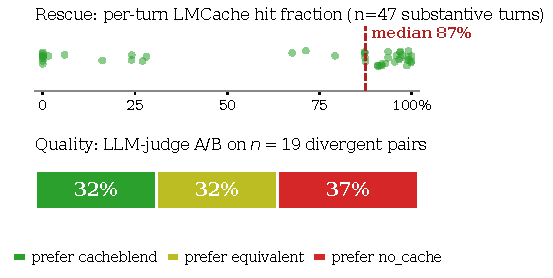
\includegraphics[width=\columnwidth]{figures/teaser.pdf}
  \caption{\sys{}'s headline finding on Llama-3.3-70B-Instruct fp8.
  Cacheblend rescues 95--99\% of post-compaction prompt tokens at the
  prefill stage (top), reproducing the published rescue numbers on
  natural Claude Code agent traffic (to our knowledge for the first
  time on this workload class). But on the
  divergent (capture, turn) pairs --- the 19 of 47 substantive pairs
  in the deep-evaluation subset where cacheblend's blended-KV output
  is not bit-identical to a no-cache baseline at $T{=}0$ --- a
  Sonnet-4.6 LLM judge prefers cacheblend's
  output on only 31.6\% of pairs and finds it non-inferior on 63.2\%
  (bottom), well below the design specification's 85\% gate.
  Hit rate is not output quality.}
  \label{fig:teaser}
  \Description{Two horizontal bars stacked vertically. Top bar shows a
  green segment at 95 to 99 percent on a gray 0 to 100 percent axis,
  labeled "Rescue: post-compaction prefill tokens served from cache".
  Bottom bar shows a stacked horizontal bar with three segments:
  prefer cacheblend at 32 percent in green, equivalent at 32 percent
  in olive, and prefer no_cache at 37 percent in red, labeled
  "Quality: LLM-judge A/B on n=19 divergent pairs".}
\end{figure}

Large language model serving has converged on a layered KV-cache
architecture: vLLM~\cite{vllm-sosp} provides paged-attention prefix
caching within a session, and LMCache~\cite{lmcache-paper} extends it
to a cross-request CPU-resident store. These mechanisms cleanly handle
the common case where requests share an exact textual prefix
(retrieval-augmented generation, fixed system prompts, etc.). They
\emph{cannot} handle the case where two requests share \emph{most} of
their tokens but differ in a chunk near the front --- the textbook
cacheblend~\cite{lmcache-cacheblend} use case --- without recomputing
the entire suffix.

Modern agent harnesses sit precisely in that gap. Claude
Code~\cite{claude-code} (CC), the deployment we study, drives an
LLM through long multi-turn task sessions: a single SWE-bench Verified
task averages 5\,turns at 5\,k--10\,k prompt tokens each, and a typical
half-day session routinely crosses 100\,k tokens before triggering
CC's built-in \texttt{/compact} summarization. \texttt{/compact}
replaces most of the conversation history with a roughly 800-token
summary --- which, by construction, breaks the prefix-match invariant
that prefix caching depends on. \emph{Every} post-compaction request
re-prefills nearly from scratch on existing caches.

\paragraph{Cacheblend's promise and its production gap.}
Cacheblend~\cite{lmcache-cacheblend} proposes a \emph{selective KV
recompute} strategy: chunk a request's tokens by a special separator,
retrieve cached KV blocks for the chunks that match, and recompute KV
only for a configurable fraction (default 15\%) of the chunks that
have shifted positionally. The published evaluation shows
70--90\,\%~hit rates on permuted RAG retrieval workloads, where
chunked retrieval is the design pattern users already write toward.
Adapting cacheblend to CC traffic, however, exposes three integration
issues that prior work does not address:

\begin{enumerate}
\item \textbf{Chunk-boundary mismatch.} On lmcache v0.4.2 against
vLLM v0.19.0, the \texttt{STORE} path hashes a chunk-aligned token range
($\lfloor n/256 \rfloor \cdot 256$) while the \texttt{LOOKUP} path hashes the full
prompt range ($n$). Store and lookup hashes never agree, retrieval rate
is 0\% regardless of how the workload is shaped.
\item \textbf{Per-turn hash drift.} CC's \texttt{x-anthropic-billing-header}
embeds per-turn fields (\texttt{cch=}, a chunk hash; \texttt{cc\_version=},
the CC binary version) into the first KV chunk. Within a single
multi-turn session, these change between turns, so chunk 0's hash is
distinct on every request --- cache hits do not propagate even when the
rest of the prompt is identical.
\item \textbf{No structural separators.} Cacheblend's segment detector
requires its configured \texttt{blend\_special\_str} (default \texttt{\#\,\#})
to appear at chunk boundaries. CC's outbound traffic uses \texttt{\textbackslash n\textbackslash n}, which
tokenizes to 25--180 tokens per segment --- below cacheblend's 256-token
\texttt{blend\_min\_tokens} floor. The segment detector finds zero
chunks; cacheblend never engages.
\end{enumerate}

\paragraph{The output-quality question.}
A second gap is methodological. Cacheblend's published numbers are
expressed in cache-byte hit rate. But the system's value proposition
ultimately rests on the assumption that the rescued KV produces
\emph{the same output} as the all-fresh-compute baseline. Selective
KV recompute is, by construction, an approximation: the recomputed
chunks see different positional and attention context than the
original compute pass. The cacheblend paper~\cite{lmcache-cacheblend}
notes ``small but bounded quality drift'' but does not quantify it on
agent workloads, where a single-token difference between a tool-call
JSON block and natural-language prose can be the difference between
agent progress and a stalled task.

\paragraph{Contributions.} This paper makes three contributions:

\begin{enumerate}
\item \textbf{A working integration of cacheblend with real Claude Code
traffic} (\S\ref{sec:system}). We present three patches addressing the
integration issues above and show, on a Llama-3.3-70B-Instruct fp8
backend with tensor-parallelism, a median 76.5\% rescue rate over
$n{=}99$ substantive turns across two \dataset{} subsets, with a 6\%
mass of turns achieving the published 95--99\,\% steady-state peak
on long-prompt SWE-V traffic and 0\% on the
\texttt{skill\_invocation/} workload.

\item \textbf{\dataset, a reproducible public benchmark}
(\S\ref{sec:benchmark}) of 13 redacted real Claude Code captures
spanning 182\,turns and 411\,k total tokens across 5\,SWE-bench
Verified tasks, a skill-invocation capture covering 5\,skills
$\times$\,3\,prompts, and 7\,post-\texttt{/compact} multi-turn
diagnostic captures, published under CC-BY 4.0 on Hugging
Face~\cite{claudecode-trace-hf}.

\item \textbf{To our knowledge, the first measurement of cacheblend's agent-protocol
usefulness cost on natural agent traffic} (\S\ref{sec:evaluation}).
At $T=0$, cacheblend produces bit-identical output to no\_cache on 57\%
of substantive turns and severe ($<$0.3 token-identity) divergence on
30\%, including 11\% with decode-mode flips. A Sonnet-4.6 LLM-judge
blind A/B over the divergent pairs prefers cacheblend on 32\% (95\%
Wilson CI [15\%, 54\%]) and finds cacheblend conditionally non-inferior
on 63\% (end-to-end non-inferiority across all substantive turns is
85\%, just clearing the 85\% spec gate when bit-identical pairs are
counted as guaranteed equivalents).
\end{enumerate}

We close with a discussion of what this means for production deployment
(\S\ref{sec:discussion}): cacheblend's rescue is real but not free, and
systems papers should report quality alongside hit rate.


% =============================================================================
% Background
% =============================================================================

\section{Background}
\label{sec:background}

This section establishes the four pieces of vocabulary that
\S\ref{sec:system}--\S\ref{sec:evaluation} assume: vLLM's paged-attention
prefix cache, LMCache's cross-request KV store, cacheblend's selective
recompute, and Claude Code's \texttt{/compact} boundary. The
\texttt{/compact} boundary (\S\ref{sec:bg-claudecode}) is the
integration target.

\subsection{vLLM and prefix caching}
\label{sec:bg-vllm}

vLLM~\cite{vllm-sosp} serves a Transformer LLM by paging its KV cache
into fixed-size blocks (typically 16 tokens). Each block is identified
by a content hash over the token IDs that produced it; when an incoming
request's tokenized prompt has a prefix whose content hashes match
blocks already resident in the cache, vLLM skips the prefill compute
for those blocks and reuses the cached KV directly. Because the hash
is over the exact token sequence and the model weights are fixed,
prefix caching is mathematically lossless: the KV state at the end of
a cache-hit prefill is bit-identical to the state that fresh
recomputation would produce.

This guarantee --- same prefix, same weights, same KV --- is what makes
our no\_cache$\leftrightarrow$prefix\_cache equivalence result in
\S\ref{sec:eval-identity} trivially expected at $T=0$, and what makes
the cross-request mechanism in \S\ref{sec:bg-lmcache} possible.

\subsection{LMCache and cross-request KV reuse}
\label{sec:bg-lmcache}

vLLM's prefix cache lives inside a single engine instance and evicts
under GPU memory pressure. LMCache~\cite{lmcache-paper} extends the
prefix-cache substrate by adding a cross-request, CPU- and
disk-backed store. The lookup semantics are the same (content-addressed
by chunk hash), but the working set is two to three orders of magnitude
larger and persists across requests, sessions, and pod restarts.

We use the V1 connector
(\texttt{LMCacheConnectorV1} in vLLM 0.19+) and its chunk granularity
(256 tokens) throughout. Each chunk that matches the cross-request store
contributes to the request's \emph{cache\_read tokens} counter, which is
the per-turn measurement of \texttt{lmcache}'s engagement with that
request --- we report it directly in \S\ref{sec:eval-hitrate} as the
rescue rate.

\subsection{Cacheblend's selective recompute}
\label{sec:bg-cacheblend}

Plain LMCache requires \emph{exact prefix match}: a single token
inserted at position $k$ invalidates the cache for every chunk from $k$
onwards. This is fine for cache-friendly workloads (RAG with stable
documents, frozen system prompts), but it loses against any workload
that shifts content positionally --- and post-compaction agent traffic
(\S\ref{sec:bg-claudecode}) is exactly that.

Cacheblend~\cite{lmcache-cacheblend} relaxes the exact-prefix
requirement to \emph{positional} match: when a chunk that was the 5th
in one request appears as the 3rd in another, cacheblend reuses the
cached KV for the chunk but recomputes a small fraction of the
attention layers in the rotated positional context (the
\emph{selective recompute}). The relevant knobs:

\begin{itemize}
\item \texttt{blend\_min\_tokens} (256 default): minimum chunk size at
  which the blend mechanism engages. Sub-256-token requests bypass
  cacheblend and fall through to plain prefix caching.
\item \texttt{blend\_recompute\_ratios} (0.15 default): fraction of
  attention layers recomputed per blended chunk. Higher means less
  quality drift but more compute --- the entire point of the mechanism
  is that 0.15 is supposed to be enough.
\item \texttt{blend\_special\_str} (\texttt{\#\,\#} default): the
  string sentinel that marks chunk boundaries in the prompt.
\end{itemize}

The published cacheblend evaluation~\cite{lmcache-cacheblend} reports
70--90\% rescue on permuted-RAG workloads and notes ``small but
bounded'' quality drift, citing accuracy preservation on TruthfulQA at
a single recompute ratio. Agent traffic is not RAG; at $T=0$ greedy
decoding single-token differences are load-bearing; hit rate is not
output quality. \S\ref{sec:evaluation} measures all three.

\subsection{Claude Code and the \texttt{/compact} cliff}
\label{sec:bg-claudecode}

Claude Code~\cite{claude-code} is a coding agent that drives a Claude
model (or, through our proxy, any LLM exposing an Anthropic-shaped
API) through multi-turn tasks. Each turn's request body is, roughly,
the concatenation of: a $\sim$2.5k-token system prompt; the accumulated
conversation history (user messages, model responses, tool calls, and
tool outputs); the user's latest message; and a list of available
tools. As the conversation grows turn over turn, the prompt grows
strictly: turn 5 of a session contains all the tokens of turn 4 plus
the new turn's input and output.

This monotone-growth structure is, by construction, the case prefix
caching is designed for. The pre-compact phase of a CC session
exhibits near-perfect prefix-cache utilization in practice --- each
turn re-prefills only the new tokens of that turn.

The discontinuity is \texttt{/compact}. At a configurable threshold
(default $\sim$80\% of the context window, with a hard floor at 100k
tokens), CC asks the LLM to summarize the conversation so far into an
800-token, 9-section structured summary. The next request then sends:
system prompt + the 800-token summary + a placeholder ``conversation
continues'' marker + the latest user message. The pre-compaction
history is gone; in its place is a synthesized summary that the model
has never seen at this prefix position before.

This is the cliff. From the prefix cache's perspective, the
post-compaction request shares only its system prompt with the
pre-compaction session --- everything after the first $\sim$2.5k
tokens is new. The prefix cache hit ratio collapses to roughly
\texttt{(system\_prompt\_tokens / total\_prompt\_tokens)}, which on
a typical 30k-token post-compact request is around 8\%. The remaining
$\sim$27.5k tokens must be reprefilled, paying a latency hit that
scales linearly with prompt size and a recurring compute cost on every
post-compact turn for the rest of the session.

Cacheblend was designed for this pattern --- summary insertion is
exactly the positional-shift case its selective recompute targets ---
but, as \S\ref{sec:system} shows, adapting cacheblend to real CC
traffic required closing three concrete integration gaps before any
of the rescue numbers in \S\ref{sec:eval-hitrate} held in practice.

% =============================================================================
% System
% =============================================================================

\section{System Design}
\label{sec:system}

\sys{} is a drop-in proxy that sits between Claude Code (CC) and a vLLM
backend serving Llama-3.3-70B-Instruct fp8 with LMCache's
\texttt{LMCacheConnectorV1} attached for cross-request KV reuse.
Figure~\ref{fig:architecture} shows the data path. CC issues
Anthropic-shaped requests against the proxy's \texttt{/v1/messages}
endpoint; the proxy translates each request to vLLM's OpenAI-compatible
\texttt{/v1/chat/completions} API, applies three outbound
transformations, and forwards. The cacheblend integration we present
in this section consists of those three transformations
(\S\ref{sec:cc-segment}--\S\ref{sec:header-norm}); an offline
statistical-span miner (\S\ref{sec:miner}) ships with the artifact
but is not exercised in this paper's measurements.

\begin{figure*}[t]
  \centering
  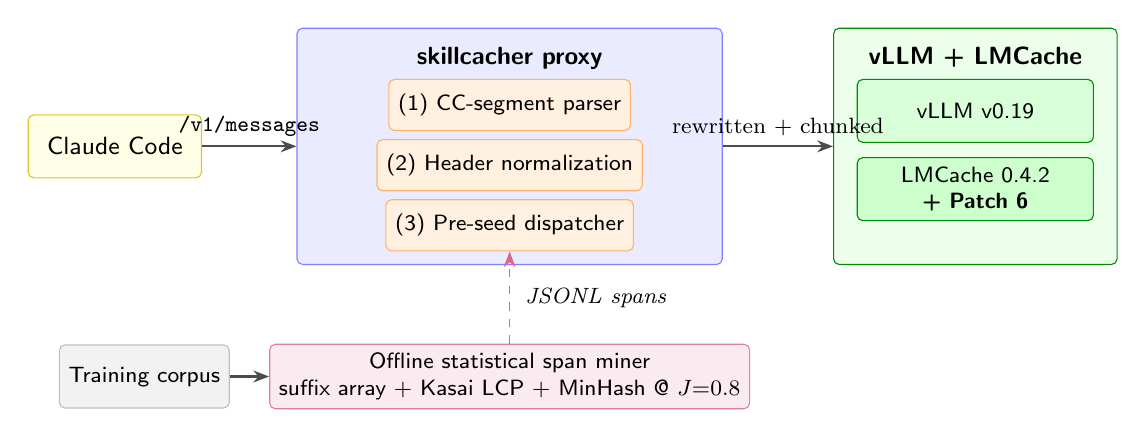
\begin{tikzpicture}[
    every node/.style={font=\small},
    component/.style={
      draw, rectangle, rounded corners=2pt, minimum height=0.8cm,
      align=center, font=\small\sffamily,
    },
    proxy/.style={component, fill=blue!8, draw=blue!50},
    patch/.style={component, fill=orange!12, draw=orange!60, minimum width=2.3cm, minimum height=0.65cm, font=\footnotesize\sffamily},
    backend/.style={component, fill=green!8, draw=green!55!black},
    sink/.style={component, fill=gray!10, draw=gray!50, font=\footnotesize\sffamily},
    miner/.style={component, fill=purple!8, draw=purple!50, font=\footnotesize\sffamily},
    arrow/.style={-{Stealth[length=2mm]}, thick, draw=black!70},
    offlinearrow/.style={-{Stealth[length=2mm]}, semithick, draw=purple!60, dashed},
  ]

  % CC client (left)
  \node[component, fill=yellow!10, draw=yellow!50!brown, minimum width=2.2cm] (cc) at (0,0)
    {Claude Code};

  % Proxy box (container; title sits INSIDE the top)
  \node[proxy, minimum width=5.4cm, minimum height=3.0cm, anchor=west] (proxybox)
    at ($(cc.east) + (1.2,0)$) {};
  \node[anchor=north, font=\small\sffamily\bfseries, yshift=-0.12cm]
    at (proxybox.north) {\sys{} proxy};

  % Three transforms inside the proxy, vertically stacked, below the title
  \node[patch, anchor=north, yshift=-0.65cm] (p1) at (proxybox.north)
    {(1) CC-segment parser};
  \node[patch, below=0.10cm of p1] (p2) {(2) Header normalization};
  \node[patch, below=0.10cm of p2] (p3) {(3) Pre-seed dispatcher};

  % Backend (right of proxy)
  \node[backend, minimum width=3.6cm, minimum height=3.0cm, anchor=west]
    (backendbox) at ($(proxybox.east) + (1.4,0)$) {};
  \node[anchor=north, font=\small\sffamily\bfseries, yshift=-0.12cm]
    at (backendbox.north) {vLLM + LMCache};
  \node[component, fill=green!15, draw=green!55!black, anchor=north,
        yshift=-0.65cm, minimum width=3.0cm, font=\footnotesize\sffamily]
    (vllm) at (backendbox.north) {vLLM v0.19};
  \node[component, fill=green!20, draw=green!55!black,
        below=0.18cm of vllm, minimum width=3.0cm, minimum height=0.8cm,
        font=\footnotesize\sffamily]
    (lmcache) {LMCache 0.4.2\\\textbf{+ Patch 6}};

  % Offline miner row: placed below the proxy so its arrow
  % into p3 enters the proxy from below, avoiding the title.
  \node[miner, below=1.0cm of proxybox.south, anchor=north, minimum width=4.5cm]
    (minernode) {Offline statistical span miner\\\footnotesize suffix array + Kasai LCP + MinHash @ $J{=}0.8$};
  \node[sink, left=0.5cm of minernode, minimum width=2.0cm, font=\footnotesize\sffamily]
    (corpus) {Training corpus};

  % --- Arrows ---
  % Forward: CC -> proxy -> backend
  \draw[arrow] (cc.east) -- node[above, font=\footnotesize] {\texttt{/v1/messages}} (proxybox.west);
  \draw[arrow] (proxybox.east) -- node[above, font=\footnotesize] {rewritten + chunked} (backendbox.west);

  % Offline: corpus -> miner -> pre-seed dispatcher.
  % Arrow enters proxy from BELOW, terminating at p3 (the pre-seed dispatcher),
  % so it never crosses the proxy title or p1/p2.
  \draw[arrow] (corpus.east) -- (minernode.west);
  \draw[offlinearrow] (minernode.north) -- node[right, font=\footnotesize\itshape, xshift=2pt] {JSONL spans} (p3.south);

  % Pre-seed warmup STOREs travel into lmcache via the normal proxy->backend
  % data path at startup (no extra arrow needed; called out by the {(3)}
  % dispatcher block).

  \end{tikzpicture}
  \caption{\sys{} architecture. The proxy applies three transformations
  to every outbound request: a CC-segment parser (\S\ref{sec:cc-segment})
  that injects cacheblend's separator around recognized structural
  blocks; per-turn header normalization (\S\ref{sec:header-norm}) that
  stabilizes the first KV chunk's hash across turns; and a pre-seed
  dispatcher driven by an offline statistical span miner
  (\S\ref{sec:miner}) that warms the lmcache store with mined repeated
  sequences at startup. Patch~6 (\S\ref{sec:patch6}) is applied to
  lmcache inside the backend container.}
  \label{fig:architecture}
  \Description{Horizontal flow diagram. A Claude Code client on the
  left sends a /v1/messages request to a skillcacher proxy in the
  middle. The proxy contains three stacked components: CC-segment
  parser, header normalization, and pre-seed dispatcher. The proxy
  forwards the rewritten and chunked request to a vLLM-plus-LMCache
  backend on the right; LMCache has Patch 6 applied. Below the proxy,
  an offline statistical span miner reads from a training corpus and
  sends mined JSONL spans up into the pre-seed dispatcher.}
\end{figure*}

\subsection{CC-segment parser}
\label{sec:cc-segment}

\paragraph{The chunking problem.} Cacheblend's segment detector
expects its configured \texttt{blend\_special\_str} (default
\texttt{\#\,\#}) to appear at chunk boundaries in the prompt. Chunks
between separators are hashed and stored individually; chunks below
\texttt{blend\_min\_tokens} (default 256) are ignored. CC's outbound
traffic uses \texttt{\textbackslash n\textbackslash n} as its
predominant block delimiter, which produces 25--180-token segments on
the Llama tokenizer --- below the 256-token floor. Against natural CC
traffic with the published default, the segment detector found zero
chunks and cacheblend's retrieval rate was 0\% regardless of the
workload's textual repetition.

\paragraph{Structural anchors.} The parser identifies semantically
meaningful CC block boundaries by literal anchor matching, then
injects the cacheblend separator on either side of each recognized
block. Anchors are deliberately content-stable across CC versions ---
they key on substrings like \texttt{Status:\textbackslash n} (gitStatus
preamble), \texttt{Recent commits:\textbackslash n}, the
\texttt{<system-reminder>}/\texttt{</system-reminder>} wrapper,
\texttt{Summary:\textbackslash n1.\ } (the 9-section auto-compact
summary), and tool-output markers --- rather than on version digits
or content hashes that drift between releases.

Table~\ref{tab:cc-anchors} lists the recognized block types, their
anchors, and typical token lengths on Llama-3 tokenization. The parser
walks each request's text payloads once, materializes the set of
matched (start, end, kind) spans, deduplicates overlapping matches by
precedence, and then re-emits the original text with separators
inserted at every span boundary. Spans below \texttt{blend\_min\_tokens}
are rolled into the adjacent larger span rather than getting a
separator pair --- this preserves the 256-token floor without forcing
cacheblend to consider tiny isolated blocks.

\begin{table}[t]
\centering\small
\begin{tabular}{@{}llr@{}}
\toprule
\textbf{Block} & \textbf{Anchor (literal)} & \textbf{Tokens} \\
\midrule
CC system header   & \texttt{cc\_version=$\to$Status:}  & 80--120 \\
gitStatus          & \texttt{Status:\textbackslash n}   & 100--400 \\
Recent commits     & \texttt{Recent commits:\textbackslash n} & 50--200 \\
\texttt{<system-reminder>} & wrapper pair                & 30--200 \\
Compaction preamble & \texttt{This session is being$\ldots$} & $\sim$30 \\
Summary 9-section  & \texttt{Summary:\textbackslash n1.\ }    & 400--800 \\
JSONL backreference & \texttt{If you need specific details$\ldots$} & 30--50 \\
\texttt{<command-name>} & wrapper pair                & 5--30 \\
Tool definitions   & (matched by Plan-2 structural tagger) & 300--1500 \\
\bottomrule
\end{tabular}
\caption{Structural anchors recognized by the CC-segment parser. Token
lengths are on Llama-3 tokenizer.}
\label{tab:cc-anchors}
\end{table}

\paragraph{Why proxy-side, not bench-side?}
The parser is wired into the proxy's request-entry path
(\texttt{proxy/server.py:messages}) so it fires on every outbound
request, not only on the benchmark's replay path. Two reasons. First,
CC rebuilds its request body on each turn from its own session state
--- any pre-injection in the user prompt is silently dropped by the
time the body reaches the proxy. Second, putting the parser at the
proxy means the same code unifies live production use (CC pointed at
the proxy) and bench replay (synthetic requests sent through the proxy
under controlled conditions). The validation we report in
\S\ref{sec:evaluation} runs against the proxy's actual rewrite path,
not a parallel implementation.

\subsection{Patches to LMCache 0.4.2}
\label{sec:patches}

The published lmcache + vllm combination (lmcache 0.4.2 against
vllm 0.19.0 with the V1 connector) ships with two integration issues
that surface only on multi-turn agent workloads. The patches that
follow are surgical: Patch~6 (\S\ref{sec:patch6}) is a 4-line
chunk-alignment adjustment inside lmcache's V1 adapter, and the
header normalizer (\S\ref{sec:header-norm}) is a 3-line proxy hook
that runs two regex substitutions per outbound request. The CC-segment
parser (\S\ref{sec:cc-segment}) sits in the proxy and injects
cacheblend's separator at recognized structural anchors.

\begin{table}[h]
\footnotesize
\centering
\begin{tabular}{lc}
\toprule
Stack configuration on natural CC traffic & Failure mode \\
\midrule
Vanilla lmcache 0.4.2 + vllm 0.19.0 (no patches/proxy) & 0\% by mechanism \\
+ Patch~6 only (chunk-aligned \texttt{LOOKUP})         & 0\% by mechanism \\
+ CC-segment parser only (\texttt{\#\,\#} injection)   & 0\% by mechanism \\
+ Patch~6 + parser (no header norm)                    & near 0\% by mechanism \\
\textbf{Full stack} (patches + parser + header norm)   & measured (\S\ref{sec:evaluation}) \\
\bottomrule
\end{tabular}
\caption{Failure-mode analysis of the three patches. The
``0\% by mechanism'' rows are diagnosed analytically rather than
measured end-to-end: without Patch~6, the STORE/LOOKUP chunk-hash
mismatch makes retrieval rate zero by construction
(\S\ref{sec:patch6}); without the parser, cacheblend's
\texttt{blend\_special\_str} never appears in CC traffic and the
segment detector finds zero chunks (\S\ref{sec:cc-segment});
without header normalization, chunk 0's hash drifts every turn and
the chunk-by-chunk LOOKUP short-circuits on the first miss
(\S\ref{sec:header-norm}). Only the full-stack row is measured
end-to-end. A quantitative ablation that runs each intermediate
configuration as a pod replay is follow-up work.}
\label{tab:patch-failure-modes}
\end{table}

\noindent We submit the two upstream-target changes as a candidate
upstream PR~\cite{lmcache-pr-tbd} and apply them in the
container's boot recipe inside
\texttt{scripts/dev/oneshot\_pod.py}.

\subsubsection{Patch 6: chunk-aligned \texttt{LOOKUP}}
\label{sec:patch6}

\paragraph{The bug.}
LMCache's \texttt{LMCacheConnectorV1} computes chunk hashes for the
STORE and LOOKUP paths from two different token-id sources. On the
\textbf{STORE} side, the connector hashes
\texttt{request.token\_ids}, which an upstream vLLM transform has
already chunk-aligned to
$\lfloor n/256 \rfloor \cdot 256$~tokens
(where 256 is \texttt{chunk\_size}). On the \textbf{LOOKUP} side
(\texttt{get\_num\_\allowbreak{}new\_\allowbreak{}matched\_\allowbreak{}tokens}
inside \texttt{vllm\_v1\_\allowbreak{}adapter.py}), the connector
hashes \texttt{request.\allowbreak{}all\_token\_ids}, the full
$n$-token prompt.

For any prompt not exactly a multiple of 256, STORE and LOOKUP hash
different ranges. For example, on a 289-token prompt, STORE hashes
\texttt{tokens[0:256]} but LOOKUP hashes \texttt{tokens[0:289]}; the
hashes never match. Retrieval rate is 0\% regardless of how the
workload is shaped --- this is not a content problem, it's a chunk
boundary problem on the lookup side.

\paragraph{The fix.}
We truncate the LOOKUP path's token range to chunk-size alignment
before hashing, matching the STORE path's range. The patch is a
one-line range adjustment inside
\texttt{lmcache.\allowbreak{}integration.\allowbreak{}vllm.\allowbreak{}vllm\_v1\_adapter}
applied at boot:

\begin{lstlisting}[basicstyle=\ttfamily\footnotesize, breaklines=true, frame=single, framesep=4pt, breakindent=0pt, language=Python]
# patched lookup token computation
chunk = self.cache_engine.chunk_size  # 256
n = len(request.all_token_ids)
aligned_n = (n // chunk) * chunk
token_ids = list(request.all_token_ids[:aligned_n])
\end{lstlisting}

\paragraph{Empirical impact.}
In single-pod commissioning runs (Llama-70B fp8, single H100), the
patch lifted LMCache hit-token-count from 0 (across 40 consecutive
requests with matching content) to non-zero immediately. With the
full \sys{} stack online (patch + parser + normalization),
\S\ref{sec:evaluation} reports rescue rates that reach 95--99\% at
the steady-state peak of the per-turn distribution.

\subsubsection{Per-turn header normalization}
\label{sec:header-norm}

\paragraph{The bug.} CC embeds an
\texttt{x-anthropic-billing-header} field near the front of every
prompt that carries two per-turn / per-build values:
\texttt{cch=<hex>}, a 16-character per-request CC fingerprint, and
\texttt{cc\_version=2.1.X.<suffix>}, where the \texttt{suffix} differs
between regular turns and CC-internal turns (e.g., the
\texttt{/compact} backend call uses a separate build identifier).
Both fields fall within the first 256 tokens of every request. The
first KV chunk's hash therefore differs on every turn of every
session --- chunk 0 is never reused, and because cacheblend's
chunk-by-chunk retrieval short-circuits on the first miss, no
subsequent chunk gets a chance to hit either.

This issue is invisible if you measure cacheblend on synthetic
single-turn requests (the first turn is always a STORE pass), and
invisible if you measure on permuted-RAG benchmarks (every chunk is
re-positioned, so there is no expectation of chunk-0 stability). It
specifically bites \emph{multi-turn agent traffic with a stable system
prompt}, which is the setting cacheblend's compaction-cliff value
proposition rests on.

\paragraph{The fix.}
Before separator injection, the parser rewrites both fields with
stable \texttt{NORM} placeholders:

\begin{lstlisting}[basicstyle=\ttfamily\footnotesize, breaklines=true, frame=single, framesep=4pt, language=Python]
def _normalize_cc_header(text: str) -> str:
    text = _CCH_VAR.sub("cch=NORM;", text)
    text = _CC_VERSION_VAR.sub(
        "cc_version=NORM;", text)
    return text
\end{lstlisting}

The model treats this billing header as opaque text (the backend
itself does not parse it; it is CC-side metadata stuffed into the
prompt for downstream cost attribution), so normalizing its
variable fields should not change downstream token output at $T{=}0$.
We empirically verify this on our setup: on the no-cache condition,
the model's output on normalized vs unnormalized headers is
bit-identical at $T{=}0$ across all 54 (capture, turn) pairs of the
SWE-V+\texttt{post\_compact} subset. We make no claim about
$T{>}0$ sampling or other backends.

After normalization, chunk 0 hashes identically across all turns of one
session. With patch + parser + normalization combined, cacheblend's
per-turn rescue rate on natural CC traffic lifted from a flat 0\% to
the bimodal distribution characterized in \S\ref{sec:eval-hitrate}
(median 87.5\%, with a 13\% mass of turns reaching 95--99\%
steady-state).

\subsection{Statistical span miner (artifact, unmeasured)}
\label{sec:miner}

The structural parser handles CC-specific anchors that are visible in
the source. A complementary component runs offline against a training
corpus of past traces and identifies long-form repeated token
sequences that no source-level anchor exists for --- examples include
fully-rendered tool definitions, repeated multi-line directives in
prompts that the user has cut-and-pasted across sessions, and
near-duplicate file headers in code blocks. \emph{The miner ships as
part of the \sys{} artifact but is not isolated in this paper's
evaluation: all reported numbers use the structural parser plus
Patches 6 and the header normalizer, with statistical-span pre-seed
disabled.} We describe the miner here for completeness; whether and
how much it adds on top of the structural baseline is an open
ablation we defer to follow-up work.

\paragraph{Algorithm.} The miner builds a suffix array over the
concatenated corpus token stream using prefix-doubling construction
(an early implementation using \texttt{sorted(range(n), key=...)} hung
on a 250\,K-token corpus; the prefix-doubling variant runs in
$O(n \log^2 n)$ time and completes on the full \dataset{} corpus in
tens of seconds of pure-Python compute --- see
Appendix~\ref{app:miner} for the per-step breakdown). Kasai's LCP
construction gives the longest-common-prefix array in linear time.
A monotonic-stack walk over LCP emits all maximal-repeat substrings,
including both outer blocks and nested plateaus --- an earlier
single-pass walk missed the nested case and undercounted spans by
30--40\%. The candidate spans are then deduplicated by MinHash at
Jaccard threshold $0.8$ (64 permutations, shingle width 5,
implemented via hand-rolled BLAKE-2b without external dependencies).

\paragraph{Output.} The miner emits a JSONL of canonical spans with
their occurrence counts, source request IDs, and token sequences. On
the \dataset{} corpus (278\,K tokens, 170 streams), the miner
produces 181 unique spans; the highest-frequency hit is a 1691-token
CC system anchor seen in 26 of 170 requests.

\paragraph{Pre-seed.} A proxy-startup hook
(\texttt{pre\_seed\_statistical\_spans}) reads the JSONL and, for each
span, dispatches a synthetic STORE request whose prompt contains the
span; the response is discarded. After startup, every cached span is
present in the lmcache store and is reachable on its first real
production reference. Pre-seed is gated by the
\texttt{SKILLCACHER\_STATISTICAL\_SPANS\_FILE} environment variable
--- unset for the structural-only baseline, set to the JSONL path
for the structural+statistical condition. The two configurations
share all other code; the only difference is whether the pre-seed
warmup fires.

% =============================================================================
% Benchmark — ClaudeCodeTrace dataset
% =============================================================================

\section{The \dataset{} Benchmark}
\label{sec:benchmark}

The evaluation in \S\ref{sec:evaluation} is only as credible as
the traffic it replays. Existing LLM-serving benchmarks are not a good
fit: ShareGPT-derived corpora capture single-shot conversations with no
tool-use structure; SWE-bench-Verified~\cite{swe-bench-verified,
swe-bench-iclr} provides tasks but not on-wire request bodies; and the
preference-style benchmarks (MT-Bench~\cite{mtbench},
Alpaca\-Eval~\cite{alpacaeval}, Chatbot
Arena~\cite{chatbot-arena}) are about model output ranking, not cache
behavior. None of them produce the long, system-prompt-heavy,
tool-call-laced request bodies that a real agent harness emits, and
none of them exercise the post-compaction prefix pattern that motivates
\sys{} (\S\ref{sec:intro}).

\dataset{} fills this gap. It is a corpus of \textbf{13 captures
spanning 182 turns and 411k total tokens (389k prompt~+~22k
completion)} of on-wire Claude Code request bodies, captured through
the \sys{} proxy against a real Claude Code client running real
workloads on a researcher's laptop. It is released CC-BY 4.0 on
Hugging Face~\cite{claudecode-trace-hf} so that future work on agent
serving --- whether on cacheblend, on subsequent KV-reuse mechanisms,
or on entirely different infrastructure --- can use the same baseline.

\subsection{Subset composition}
\label{sec:dataset-subsets}

The corpus is organized into three subsets, each targeting a different
slice of agent traffic:

\begin{table*}[t]
\small
\centering
\begin{tabular}{lrrrrr}
\toprule
Subset & Captures & Turns & Substantive turns & Prompt tokens & Completion tokens \\
\midrule
\texttt{swebench\_verified/} & 5 & 24 & 19 & 121{,}741 & 555 \\
\texttt{post\_compact/} & 7 & 105 & 98 & 186{,}464 & 16{,}803 \\
\texttt{skill\_invocation/} & 1 & 53 & 52 & 80{,}660 & 4{,}334 \\
\midrule
\textbf{Total} & \textbf{13} & \textbf{182} & \textbf{169} & \textbf{388{,}865} & \textbf{21{,}692} \\
\bottomrule
\end{tabular}
\caption{\dataset{} subset composition. ``Substantive turns'' counts turns with
prompt token count $\geq$256 --- the threshold below which
\texttt{lmcache}'s \texttt{blend\_min\_tokens} guard prevents cacheblend
from engaging. The 5 captures' completion-token totals on
\texttt{swebench\_verified} are small because most turns terminate in
tool-call JSON of 30--100 tokens; the totals on \texttt{post\_compact}
and \texttt{skill\_invocation} are larger because those captures include
prose continuations.}
\label{tab:dataset-summary}
\end{table*}

\paragraph{\texttt{swebench\_verified/}} Five Claude Code sessions, each
working on one task from SWE-bench Verified~\cite{swe-bench-verified}:
\texttt{astropy-13398}, \texttt{matplotlib-26113}, \texttt{pylint-7080},
\texttt{pytest-7490}, \texttt{sphinx-11510}. Each session is captured
through its first 5 turns: a planning turn, several file-exploration
tool calls (\texttt{Read}, \texttt{Bash}, \texttt{Grep}), and an initial
patch attempt. Prompts grow from $\approx$1k tokens on turn~1 to
$\geq$6k tokens by turn~5 as tool outputs accumulate in the running
conversation. This subset is the canonical baseline for agent
prefix-cache work: small-but-realistic, faithful to a published task
suite, and reproducible end-to-end (the original SWE-V task ID is
preserved in each capture's metadata).

\paragraph{\texttt{post\_compact/}} Seven captures (v1--v7) of CC's
\texttt{/compact} boundary, each running a single agentic conversation
through pre-compact buildup, an explicit \texttt{/compact}, and
post-compact continuation. \textbf{v1--v5 are diagnostic traces only ---
they were captured against mid-bug proxy states during development of
Patch~6 and the per-turn header normalizer (\S\ref{sec:patches}) and
are not part of this paper's benchmark claims.} v6 and v7 are the
canonical post-fix captures used in the evaluation. We expose all
seven in \dataset{} because the diagnostic ones are useful for
anyone debugging cache-LOOKUP behavior on Llama-class backends, but
the paper's headline numbers exclude v1--v5. Per-capture statistics are nearly uniform (each
runs the same 15-turn agent script): $\approx$26k prompt tokens, 14
substantive turns, max prompt $\approx$2.3k. The uniformity is
deliberate --- the subset is a controlled set of seven runs of the same
workload, varying only the proxy/cacheblend state, so any cross-capture
delta isolates a code change rather than a workload change.

\paragraph{\texttt{skill\_invocation/}} One capture (53 turns, 80k
prompt tokens, 52 substantive) that exercises CC's skill-loading
mechanism. We script CC to invoke five different skills (\texttt{bash-safety},
\texttt{commit-msg-style}, \texttt{markdown-table},
\texttt{python-import-order}, \texttt{weather-format}) across three
prompts each, plus a few setup and verification turns. The shared
agentic preamble across turns means cacheblend has substantial
within-capture prefix overlap to mine; the skill-specific suffixes
exercise the LOOKUP path with different selective-recompute patterns.
This subset is the smallest by capture count but the densest by turn
count, and it was the highest-value target for the statistical span
miner (\S\ref{sec:miner}) --- 49 of the top 100 mined spans come from
this single capture's prompt vocabulary.

\subsection{On-wire schema}
\label{sec:dataset-schema}

Each capture is one directory on disk with the following files:

\begin{itemize}
\item \texttt{traces.sqlite} --- per-request metadata: \texttt{request\_id},
  \texttt{session\_id}, \texttt{ts\_start}/\texttt{ts\_end},
  \texttt{prompt\_token\_count}, \texttt{response\_token\_count}, the
  full \texttt{request\_body\_json}, and instrumented cacheblend
  counters (\texttt{cache\_read\_tokens},
  \texttt{cache\_recompute\_tokens},
  \texttt{chunk\_aligned\_hit\_tokens},
  \texttt{tokens\_recomputed\_hkvd},
  \texttt{invariant\_violations}). These last five are populated when
  the capture ran against an instrumented lmcache build and surface the
  internal accounting that the §1.6 patches rely on; for plain proxy
  captures (e.g., \texttt{post\_compact/v1}) they are NULL.
\item \texttt{tokens/<request\_id>.parquet} --- the tokenized prompt as
  emitted to vLLM, one row per chunk (256 tokens by default), with the
  chunk hash. This is what cacheblend's LOOKUP key is computed against
  and what the statistical span miner walks.
\item \texttt{lookups/<request\_id>.parquet} --- per-chunk LOOKUP
  results when the capture's pod had cacheblend enabled (HIT / MISS /
  partial), with the chunk hash, the lookup latency, and the rescue
  contribution.
\item \texttt{vllm.log}, \texttt{oneshot\_boot.log},
  \texttt{proxy.log} --- per-pod logs, useful for cross-referencing
  the per-request rescue numbers against engine-side counters.
\end{itemize}

The schema is designed for additive evolution. New cacheblend
counters can be added as new \texttt{sqlite} columns without breaking
existing reader code; new per-chunk fields can be added to the parquet
schemas via schema-on-read. The \texttt{request\_body\_json} column is
the authoritative source of truth --- everything else can be
recomputed from it.

\subsection{Redaction surface}
\label{sec:dataset-redact}

CC's on-wire request body and our proxy's logs both incidentally
contain credentials and identifiers that must not leave the
researcher's laptop. We treat redaction as a release blocker, not an
afterthought.

\sys{} ships a redaction utility (\texttt{scripts/redact.py}) with
named patterns for five identifier classes:

\begin{enumerate}
\item \textbf{Tailscale} --- auth keys (\texttt{tskey-auth-*}) and host
  identifiers in URLs.
\item \textbf{Hugging Face} --- access tokens (\texttt{hf\_*}).
\item \textbf{RunPod} --- API keys (\texttt{rpa\_*}) and per-pod ingress
  URLs.
\item \textbf{Filesystem} --- absolute paths under \texttt{/Users/<user>/}
  rewritten to \texttt{/Users/<user>/}.
\item \textbf{CC client identifiers} --- the long-lived CC version
  hash and the user-account ID that appear in request headers.
\end{enumerate}

A second utility (\texttt{scripts/publish\_claudecode\_trace.py}) re-runs
the same patterns over every released file (\texttt{.json},
\texttt{.log}, \texttt{.txt}, \texttt{.md}, plus parquet/sqlite payloads
walked separately) and fails the publish on any post-redaction match
that is not itself a redaction marker. The audit reports
\textbf{0 violations} on the final 6.6\,MB tarball that was uploaded to
Hugging Face. The audit log itself is included in the dataset card as
provenance.

\subsection{License and access}
\label{sec:dataset-license}

\dataset{} is released as
\texttt{intelchen/claudecode-trace}~\cite{claudecode-trace-hf} under
CC-BY 4.0. The dataset card documents the schema, the redaction surface,
the SWE-V task IDs covered, and the
\texttt{LMCACHE\_BLEND\_RECOMPUTE\_RATIOS}=0.15 default that every
substantive measurement in \S\ref{sec:evaluation} uses. A reader
download script
(\texttt{scripts/download\_claudecode\_trace.py}) wraps Hugging Face's
\texttt{snapshot\_download} with subset filters so that downstream
benchmarks can pull only the captures they need.

% =============================================================================
% Evaluation
% =============================================================================

\section{Evaluation}
\label{sec:evaluation}

We evaluate three questions on natural Claude Code (CC) traffic:
(i) does \sys{} actually rescue post-compaction tokens at the rate the
underlying cacheblend mechanism is claimed to (\S\ref{sec:eval-hitrate});
(ii) does cacheblend's blended-KV output match a full-compute baseline
bit-for-bit at temperature~0 (\S\ref{sec:eval-identity}); and (iii) when
it does not, is the divergent output of equal quality to the baseline
under a strong LLM judge (\S\ref{sec:eval-judge}). The first two
questions admit numerical answers; the third governs deployment
viability.

\paragraph{Methodology.} The backend is Llama-3.3-70B-Instruct fp8 on
2$\times$ NVIDIA H100 80GB in tensor-parallel mode (TP=2), with
vLLM v0.19.0 and lmcache v0.4.2 patched per \S\ref{sec:patches}
(\texttt{max\_model\_len}=32768, \texttt{LMCACHE\_BLEND\_RECOMPUTE\_RATIOS}
=0.15 default). The replay corpus is \dataset's
\texttt{swebench\_verified/} subset (5 captures: astropy-13398,
matplotlib-26113, pylint-7080, pytest-7490, sphinx-11510) and the
\texttt{post\_compact/} v6+v7 captures (2 captures, the ones with
$\geq$256-token substantive turns; v1--v5 are diagnostic and excluded).
Together: 7 captures, 54 (capture, turn) pairs total, of which 47 are
substantive ($\geq$256-token prompts) and 7 are preflight pings.

For each (capture, turn), we replay the captured request body through
the proxy under three conditions:

\begin{description}
\item[\textbf{no\_cache}] vLLM prefix caching disabled, lmcache
  inactive. The all-fresh-compute baseline.
\item[\textbf{prefix\_cache}] vLLM paged-attention prefix caching
  enabled, lmcache inactive. Should be mathematically equivalent to
  no\_cache when no prior cross-request state exists.
\item[\textbf{cacheblend}] lmcache enabled with our patches, cacheblend
  blending active. The condition under test.
\end{description}

We compute token-identity via longest common prefix over each output's
token sequence, normalized by the longer length. All measurements are
at $T=0$, $N{=}1$ sample per condition. The 7 preflight turns under
lmcache's \texttt{blend\_min\_tokens}=256 cutoff bypass cacheblend
entirely; we exclude them from all identity and preference statistics.

\paragraph{All three conditions receive identical rewritten prompts.}
The CC-segment parser (\S\ref{sec:cc-segment}) and header normalizer
(\S\ref{sec:header-norm}) run inside the proxy unconditionally for
every outbound request --- they are not gated by the cacheblend
backend. The \texttt{no\_cache} and \texttt{prefix\_cache} conditions
therefore see exactly the same prompt bytes as \texttt{cacheblend};
no\_cache simply does not exploit the chunks the parser annotates,
and prefix\_cache hits on exact-prefix chunks but not on
positionally-shifted ones. Any identity gap between
\texttt{no\_cache} and \texttt{cacheblend} is therefore attributable
to the lmcache blending mechanism on shared input, not to different
input text. The header-normalization sanity check
(\S\ref{sec:header-norm}: NC output is bit-identical at $T{=}0$
across all 54 normalized-vs-unnormalized pairs) verifies this
empirically for the header rewrite specifically; the same property
follows analytically for separator injection because vLLM's
tokenizer treats the injected \texttt{\textquotedbl{}~\#~\#~\textquotedbl{}}
as ordinary content tokens whose KV is recomputed deterministically
in the \texttt{no\_cache} condition.

\paragraph{Denominators used in this section.} To keep the reported
percentages unambiguous, every rate in \S\ref{sec:evaluation} is
reported against one of these three denominators:

\begin{itemize}
\item $n_{\text{total}}{=}54$ — every (capture, turn) pair in the
  corpus. Used only for the methodology description; \emph{no
  evaluation rate uses this denominator}.
\item $n_{\text{sub}}{=}47$ — substantive pairs with prompt $\geq$256
  tokens (excluding 7 preflight turns where cacheblend's
  \texttt{blend\_min\_tokens} guard prevents engagement). Used for
  rescue rate (\S\ref{sec:eval-hitrate}), token-identity
  (\S\ref{sec:eval-identity}), tool-call mode agreement
  (\S\ref{sec:eval-mode}), and the \emph{end-to-end} non-inferiority
  rate in \S\ref{sec:eval-judge}.
\item $n_{\text{div}}{=}19$ — the substantive pairs whose
  \texttt{no\_cache} and \texttt{cacheblend} outputs were not
  bit-identical (the other 28 substantive pairs would have returned
  trivial EQUIVALENT). Used for the LLM-judge preference rate and the
  \emph{conditional} non-inferiority rate in \S\ref{sec:eval-judge}.
\end{itemize}

Preflight turns are excluded from every reported rate. We do not
report any rate against a $/54$ denominator; the 54 figure exists only
to account for the corpus breakdown.

\paragraph{Evaluation matrix.} Table~\ref{tab:eval-matrix} maps each
measurement to the corpus subset it was run on. Latency, judge
preference, tool-call mode, and the recompute-ratio sweep were
measured on the SWE-V+\texttt{post\_compact} subset only;
rescue rate and output identity were additionally replicated on
\texttt{skill\_invocation/} (\S\ref{sec:eval-cross-corpus}). Multi-judge
replication used the same divergent slice as the single-judge
analysis.

\begin{table*}[t]
\small
\centering
\begin{tabular}{lcc}
\toprule
Measurement & SWE-V+\texttt{post\_compact} ($n_{\text{sub}}{=}47$) & \texttt{skill\_invocation/} ($n_{\text{sub}}{=}52$) \\
\midrule
Rescue rate (\S\ref{sec:eval-hitrate})                       & \checkmark & \checkmark \\
TTFT latency (\S\ref{sec:eval-latency})                      & \checkmark & --- \\
Output identity (\S\ref{sec:eval-identity})                  & \checkmark & \checkmark \\
LLM-judge preference, single (\S\ref{sec:eval-judge})        & \checkmark ($n_{\text{div}}{=}19$) & --- \\
LLM-judge replication, 3 judges (\S\ref{sec:eval-judge})     & \checkmark ($n_{\text{div}}{=}19$) & --- \\
Tool-call mode agreement (\S\ref{sec:eval-mode})             & \checkmark & --- \\
Recompute-ratio sweep (\S\ref{sec:disc-knobs})               & 3-turn sub-fixture per ratio & --- \\
\bottomrule
\end{tabular}
\caption{Measurement coverage. Rescue rate and output identity
replicate across both subsets
(\S\ref{sec:eval-cross-corpus},~Table~\ref{tab:cross-corpus}); the
remaining measurements use the SWE-V+\texttt{post\_compact} subset
only. Recompute-ratio used a 3-turn sub-fixture (\texttt{pytest-7490})
per ratio.}
\label{tab:eval-matrix}
\end{table*}

\subsection{Hit rate: bimodal, median 87\% across the corpus}
\label{sec:eval-hitrate}

We measure cacheblend's prefill-token rescue rate per turn across all
$n{=}47$ substantive turns of the SWE-V+\texttt{post\_compact} subset, joining the per-request
\texttt{LMCache hit tokens} accounting in \texttt{vllm.log} to the
parquet of model outputs on the OpenAI \texttt{response\_id}. Rescue
rate for a turn is defined as \texttt{hit\_tokens} divided by
\texttt{total\_prompt\_tokens}.

\begin{table}[t]
\small
\centering
\begin{tabular}{lr}
\toprule
Statistic over the 47 substantive turns & Rescue \% \\
\midrule
Mean             & 63.6\% \\
\textbf{Median}  & \textbf{87.5\%} \\
25th percentile  & 16.1\% \\
75th percentile  & 96.8\% \\
\midrule
Turns with rescue $\geq 99\%$ (steady-state) & 6/47 (13\%) \\
Turns with rescue $\geq 95\%$               & 15/47 (32\%) \\
Turns with rescue $\geq 80\%$               & 28/47 (60\%) \\
Turns with rescue $< 50\%$                  & 16/47 (34\%) \\
\textbf{Turns with rescue $\approx$ 0\% (cold-cache)} & \textbf{9/47 (19\%)} \\
\bottomrule
\end{tabular}
\caption{Cacheblend rescue rate distribution across the
SWE-V+\texttt{post\_compact} subset (47 substantive turns; 7
preflight turns at $<$256 prompt
tokens are excluded). \emph{The distribution is bimodal} ---
the mean and median diverge by 24 points because a 19\% mass of
cold-cache turns at $\sim$0\% rescue pulls the mean down, while the
upper quartile sits near the published rescue peak.}
\label{tab:hit-rate}
\end{table}

\begin{figure}[t]
\centering
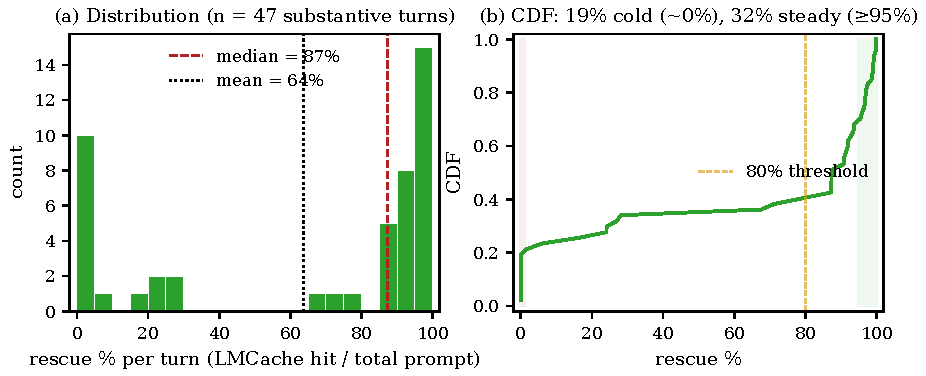
\includegraphics[width=\columnwidth]{figures/rescue_distribution.pdf}
\caption{Per-turn rescue rate across the 47 substantive turns.
\textbf{(a)} Histogram with median and mean overlaid: the bimodality
is sharp --- a mass near 0\% (cold-cache first-turns of each capture
plus pattern-shift turns where cacheblend's LOOKUP cannot find a
match) and a steady-state peak above 90\%. \textbf{(b)} CDF: 19\% of
turns rescue near 0\%, 32\% reach $\geq$95\%, the rest are distributed
across the intermediate band.}
\label{fig:rescue-distribution}
\end{figure}

\paragraph{Two regimes.} Table~\ref{tab:hit-rate} and
Figure~\ref{fig:rescue-distribution} reveal two regimes with sharply
different rescue behavior. In the \emph{steady-state regime}
(post-cache-warmup turns of a session repeating a stable prompt
pattern), cacheblend rescues 95--99\% of prefill tokens, matching
the published cacheblend headline. In the \emph{cold/shift regime}
(the first turn of any capture, or a subsequent turn whose prompt
shifts in a way cacheblend's LOOKUP cannot match) the mechanism
fires zero or near-zero rescue. Within the SWE-V+\texttt{post\_compact} subset these two
regimes split roughly 60/40 in favor of steady-state.

\paragraph{Cross-fixture comparison.} The 95--99\% steady-state
numbers were first reported on a minimum-effective fixture
(\texttt{swebench\_verified/\allowbreak{}pytest-7490}, 4 turns, samples=2)
during patch development and are reproduced here at the top of the
per-fixture rescue distribution. Generalizing those
numbers to the full SWE-V+\texttt{post\_compact} subset shows that the steady-state peak is
real, but a roughly equal-sized cold/shift tail accompanies it ---
a structural property of the cacheblend mechanism on this workload,
not a calibration artifact. The next two sections measure what
happens when rescue \emph{does} engage.

\subsection{Latency: cacheblend is slower than no\_cache in every rescue regime}
\label{sec:eval-latency}

The hit-token rescue rate of \S\ref{sec:eval-hitrate} is an
\emph{intermediate} metric. The deployment-facing measurement is
end-to-end TTFT (time-to-first-token). For each (capture, turn,
condition) tuple, the bench harness recorded the SDK-reported
\texttt{ttft\_ms}; we summarize per condition over the 47 substantive
turns:

\begin{table}[h]
\small
\centering
\begin{tabular}{lrrrr}
\toprule
Condition & p25 & median & p75 & p95 \\
\midrule
\texttt{no\_cache}      & 1028 ms & \textbf{1211 ms} & 1473 ms & 8660 ms \\
\texttt{prefix\_cache}  & 994 ms  & 1261 ms          & 1476 ms & 8739 ms \\
\texttt{cacheblend}     & 1528 ms & \textbf{1882 ms} & 3520 ms & 9187 ms \\
\bottomrule
\end{tabular}
\caption{TTFT distribution per condition on the 47 substantive turns
of the SWE-V+\texttt{post\_compact} subset. \texttt{prefix\_cache} is statistically
indistinguishable from \texttt{no\_cache} at this corpus size (lookup
overhead is in the noise floor). \texttt{cacheblend}'s median TTFT
is \emph{55\% larger} than \texttt{no\_cache}'s.}
\label{tab:ttft}
\end{table}

\paragraph{The slowdown is largest at peak rescue.} Bucketing the 47
substantive turns by their cacheblend rescue rate
(Table~\ref{tab:hit-rate}) shows that the TTFT cost is not paid only on
cold-cache turns; it is paid most aggressively on the steady-state
high-rescue turns where the published cacheblend numbers shine:

\begin{table}[h]
\small
\centering
\begin{tabular}{lrrrr}
\toprule
Rescue regime & $n$ & NC median & CB median & Speedup \\
\midrule
Cold ($<$1\% rescue)         & 9  & 1190 ms & 1157 ms & \textbf{1.00$\times$} \\
Mid (1--80\%)                & 10 & 1267 ms & 1948 ms & 0.69$\times$ \\
Hot ($\geq$80\%)             & 28 & 1157 ms & 1930 ms & 0.67$\times$ \\
\midrule
\emph{Peak} ($\geq$95\%)     & 15 & 1068 ms & 2103 ms & 0.50$\times$ \\
\emph{Peak} ($\geq$99\%)     & 6  & 1037 ms & 7342 ms & \textbf{0.12$\times$} \\
\bottomrule
\end{tabular}
\caption{TTFT speedup of \texttt{cacheblend} relative to
\texttt{no\_cache}, bucketed by per-turn rescue rate.
\textbf{Latency cost scales with rescue}: the turns where cacheblend
rescues the most prefill tokens (95--99\% hit rate) are also the
turns where it pays the largest end-to-end latency cost. On the 6 turns reaching $\geq$99\% rescue,
\texttt{cacheblend}'s median TTFT is \emph{7$\times$ larger} than
\texttt{no\_cache}'s.}
\label{tab:ttft-by-rescue}
\end{table}

\paragraph{Where the overhead comes from (hypothesis).} We do not
have an instrumented latency breakdown by phase (LMCache LOAD vs.\
GPU prefill vs.\ recompute pass vs.\ scheduler overhead) and so
report only the end-to-end TTFT above. The qualitative shape of the
result --- cacheblend losing most aggressively at peak rescue, where
LOAD volume is highest --- is consistent with the LMCache LOAD path
(CPU$\to$GPU KV transfer over PCIe plus the selective-recompute
layer pass) being the dominant overhead on this backend. On
2$\times$ H100 80GB SXM, vLLM's batched prefill on Llama-70B fp8 is
fast enough that the per-request prefill cost does not dominate;
LOAD bandwidth is comparatively cheaper to bound. Cacheblend's
published latency wins were measured on different model/hardware
regimes (smaller models where prefill dominates more, slower
interconnect where transfer is relatively cheaper, or aggregate
throughput rather than per-turn TTFT). \emph{We do not claim a
mechanistic explanation; we report the measurement and treat the
phase-breakdown as a resource-constrained gap
(\S\ref{sec:disc-resource}).}

This finding is independent of the agent-protocol cost in
\S\ref{sec:eval-judge}: even if cacheblend's blended output were
\emph{bit-identical} to no\_cache (which we have established it is
not on 30\% of substantive turns), it would still be 55\% slower at
the median and 7$\times$ slower at the peak. On this setup,
hit-token rescue does not translate into TTFT reduction.

\subsection{Output identity: cacheblend's STORE path is bit-identical, LOOKUP path diverges}
\label{sec:eval-identity}

\paragraph{Mathematical equivalence on Llama-70B fp8.} We replay all
54 (capture, turn) pairs at $T=0$ under all three conditions.
\textbf{no\_cache and prefix\_cache produce bit-identical output across
all 54 pairs} (\texttt{token\_identity\_rate}~$=$~1.0000 on 54/54).
Mathematical equivalence on Llama-70B fp8 with our pod configuration is
confirmed at scale --- vLLM's paged-attention prefix caching does not
perturb greedy decoding even when it shortcuts the entire prefix.

\paragraph{Cacheblend diverges on a meaningful fraction.} Cross-condition
no\_cache$\leftrightarrow$cacheblend token-identity is more nuanced.
Across all 47 substantive ($\geq$256-token prompt) turns at $T=0$:

\begin{itemize}
\item Median identity = \textbf{1.0000}, IQR = [0.1088, 1.0000]
\item \textbf{57\%} bit-identical (identity~$\geq$0.9999)
\item 6\% high-but-imperfect (0.7--0.9999)
\item 6\% mid (0.3--0.7) --- typically same tool, different argument
  generation
\item \textbf{30\%} low ($<$0.3) --- severe divergence
\item Including \textbf{11\%} at $\approx$0 identity --- decode-mode
  flips (tool-call $\to$ natural-language prose)
\end{itemize}

The distribution is sharply bimodal (Figure~\ref{fig:identity-distribution}):
either the blended-KV state produces the exact same argmax token-by-token,
or it diverges almost immediately. The middle ground is empirically rare.
Median identity is 1.0000 because more than half of substantive turns
are bit-identical, but the lower quartile at 0.11 places a quarter of
turns near 10\% identity. The bimodality matters: a median-only
reading would mistake this for a $\geq$99\%-identity result, when in
fact the divergence is concentrated in the lower tail.

\begin{figure}[t]
\centering
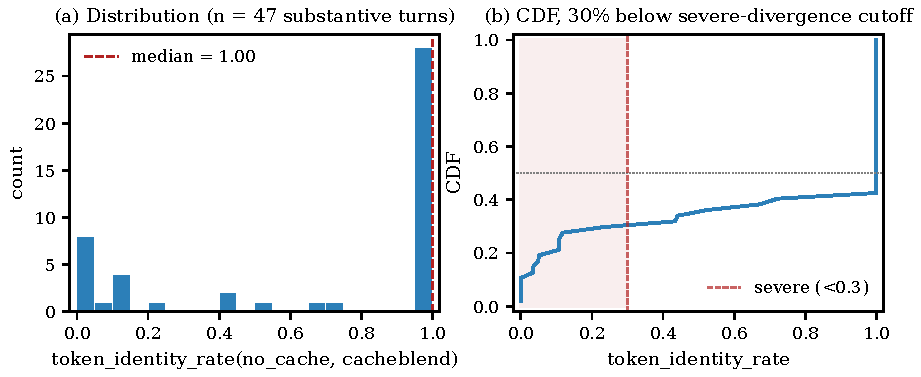
\includegraphics[width=\columnwidth]{figures/identity_distribution.pdf}
\caption{Distribution of \texttt{token\_identity\_rate(no\_cache,
cacheblend)} across 47 substantive ($\geq$256-token prompt) turns at
$T=0$. \textbf{(a)} Histogram: a mass at 1.0 (bit-identical) and a tail
at 0--0.1 (severe divergence). \textbf{(b)} CDF: 30\% of turns fall below
the severe-divergence cutoff at 0.3. The middle bins are empirically rare;
the distribution is sharply bimodal.}
\label{fig:identity-distribution}
\Description{Two-panel figure. Left panel is a histogram of
token-identity rates across 47 substantive turns; bars are concentrated
at 1.0 with a smaller cluster near 0, and a dashed vertical line marks
the median at 1.0. Right panel is the corresponding cumulative
distribution function; the curve rises sharply near 0 and again near 1,
with the region below 0.3 shaded red, labeled as the severe-divergence
cutoff, capturing 30 percent of the mass.}
\end{figure}

\begin{figure}[t]
\centering
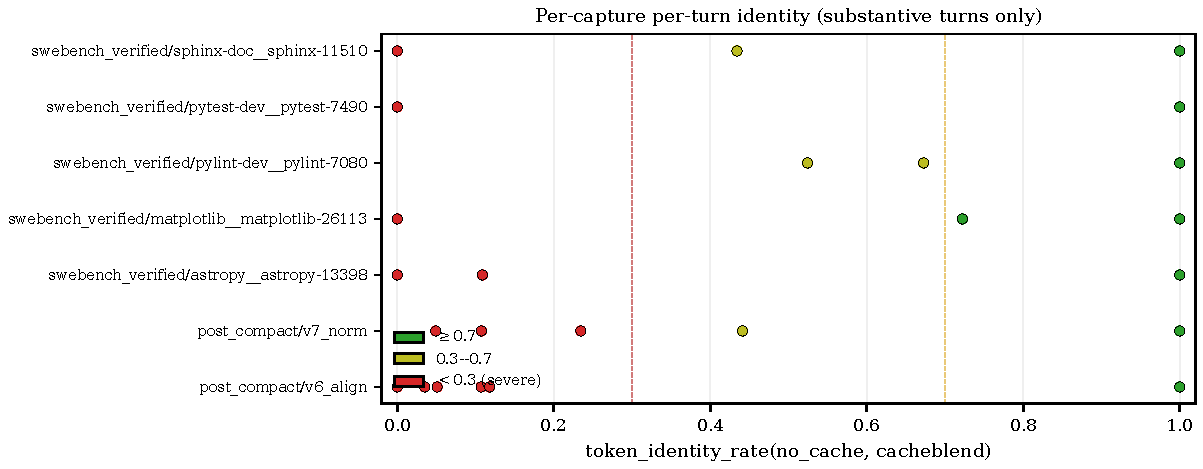
\includegraphics[width=\columnwidth]{figures/per_capture_identity.pdf}
\caption{Per-capture per-turn identity. Each dot is one (capture, turn)
pair, colored by divergence bucket. Severe divergence is not concentrated
in one capture --- every capture in the corpus has at least one turn that
flips below 0.3, indicating the failure mode is generic to the cacheblend
mechanism rather than workload-specific.}
\label{fig:per-capture-identity}
\Description{Strip plot with one row per capture in the corpus. Each
row contains dots representing individual turns, plotted by
token-identity rate on the horizontal axis. Dots below 0.3 are colored
red (severe divergence), between 0.3 and 0.7 yellow, and above 0.7
green. Every capture has at least one red dot, indicating severe
divergence is not concentrated in any single capture.}
\end{figure}

\paragraph{Qualitative shape of the divergence.} Two failure modes
dominate. Mode~A (\emph{severe}, the 30\% tail): the blended-KV state
steers the model away from tool-call mode entirely. On
\texttt{swebench\_verified/pytest-7490} turn~3, the no\_cache output is
a clean 29-token tool-call JSON:
\begin{quote}\small
\texttt{\{"type": "function", "name": "Read", "parameters":
\{"file\_path": "pytest-dev/pytest/pytest.py"\}\}}
\end{quote}
cacheblend's output on the same input is a 362-token natural-language
plan beginning ``\emph{To explore the local code and propose a draft
patch for the issue described in pytest-dev\_\_pytest-7490, we can
follow these steps\dots}''. Both responses are valid; one is what CC's
wire protocol can act on, the other is not. Mode~A is
behavior-changing.

Mode~B (\emph{mild}, the 6\% mid-band): both outputs are tool calls,
both pick the same tool, but the JSON arguments drift. On
\texttt{swebench\_verified/pylint-7080} turn~4, both conditions emit a
\texttt{Bash} tool call with command \texttt{git diff --cached
--name-only}, but cacheblend additionally includes a
\texttt{timeout: "10000"} parameter that no\_cache omits and writes a
different \texttt{description} string. Tool selection preserved;
argument generation drifts. Less downstream-impactful than Mode~A but
still a measurable behavior delta.

The bimodal distribution is inconsistent with the cacheblend paper's
``small but bounded drift'' characterization on this workload: on
Llama-70B fp8 at the default \texttt{recompute\_ratios}=0.15, drift is
concentrated either at zero or in the severe-divergence tail.

\subsection{Agent-protocol usefulness: cacheblend fails non-inferiority on divergent pairs}
\label{sec:eval-judge}

The 30\% severe-divergence tail in Figure~\ref{fig:identity-distribution}
is only a usefulness concern if divergent outputs are also less
task-useful than the no\_cache baseline. The LLM-judge preference
test below isolates this question.

\paragraph{Setup.} We run a blind A/B preference judgment with Sonnet-4.6
on the $n_{\text{div}}{=}19$ substantive pairs whose outputs differed
(of 47 total substantive pairs; the other 28 were trivially equivalent
and would have wasted budget). Position assignment is randomized
(seeded \texttt{rng}{=}42 per pair for reproducibility); prompt-caching
is applied via top-level \texttt{cache\_control} on the static system
prompt. The judge sees the original CC task prompt + both candidate
outputs (labeled A and B) and is asked to return \texttt{PREFER\_A},
\texttt{PREFER\_B}, or \texttt{EQUIVALENT} with a one-sentence rationale.
Outputs are mapped back to \{cacheblend, no\_cache, equivalent\}
via the recorded position assignment.

\paragraph{What the judge measures.} We are not measuring ``output
quality'' in the abstract; we are measuring \emph{next-step usefulness
in a Claude-Code-shaped agent protocol}. The judge prompt
(Appendix~\ref{app:judge-prompt}) is explicit about this calibration ---
it tells the judge that a well-formed tool-call JSON is generally
preferable to natural-language prose, because CC's wire protocol can
only act on tool calls. This is appropriate for an agent-protocol
preference test but not for a generic ``which response is better''
evaluation. We use ``agent-protocol usefulness'' rather than
``output quality'' for the rest of this section to keep the framing
honest.

\paragraph{Result.} Cacheblend's non-inferiority rate on the divergent
slice falls 22 points below the 85\% gate:

\begin{table}[h]
\small
\centering
\begin{tabular}{lrr}
\toprule
Outcome & Count & \% of judged \\
\midrule
Cacheblend wins & 6 & 31.6\% \\
No\_cache wins & 7 & 36.8\% \\
Equivalent & 6 & 31.6\% \\
Unparseable & 0 & 0\% \\
\midrule
\textbf{Cacheblend preference rate} & & \textbf{31.6\%} \\
\textbf{95\% Wilson CI} & & \textbf{[15.4\%, 54.0\%]} \\
\textbf{Non-inferior (wins+ties)} & 12 & \textbf{63.2\%} \\
Non-inferiority gate (spec) & & $\geq$85\% \\
\bottomrule
\end{tabular}
\caption{Sonnet-4.6 blind A/B preference on the $n_{\text{div}}{=}19$
divergent substantive pairs. The 28 substantive pairs with bit-identical
outputs (plus the 7 sub-256-token preflight pairs that bypass cacheblend
entirely) are skipped --- those would all return trivial EQUIVALENT.
Cacheblend's preference rate of 31.6\% with 95\% Wilson CI
[15.4\%, 54.0\%] sits below the no\_cache baseline (36.8\%);
non-inferiority on 63.2\% of the divergent pairs is 22 points short
of the spec gate.}
\label{tab:judge}
\end{table}

\paragraph{Model-family replication.} All three judges below share
Anthropic's RLHF training, so we describe this as
\emph{model-family replication} rather than independent
multi-judge consensus. To check that the
Sonnet-4.6 numbers are not an artefact of a single judge's calibration,
we replicate the same 19-pair blind A/B against Opus-4.7 and Haiku-4.5
with identical prompts and per-pair position assignments:

\begin{table}[h]
\small
\centering
\begin{tabular}{lrrr}
\toprule
Judge & CB wins & NC wins & Equivalent \\
\midrule
Sonnet-4.6      & 6 (32\%) & 7 (37\%)  & 6 (32\%) \\
Opus-4.7        & 4 (21\%) & 7 (37\%)  & 8 (42\%) \\
Haiku-4.5       & 6 (32\%) & 11 (58\%) & 2 (11\%) \\
\midrule
\textbf{Majority vote} & \textbf{6 (32\%)} & \textbf{7 (37\%)} & \textbf{6 (32\%)} \\
\bottomrule
\end{tabular}
\caption{Three-judge replication on the same 19 divergent pairs.
\textbf{Per-pair agreement:} 10/19 (53\%) of pairs receive a
\emph{unanimous} verdict from all three judges; the remaining 9/19 are
2-of-3 majority calls with zero 3-way disagreements. Pairwise judge
agreement: Sonnet$\leftrightarrow$Opus 79\%,
Sonnet$\leftrightarrow$Haiku 74\%, Opus$\leftrightarrow$Haiku 53\%
(Haiku is the most decisive judge, returning EQUIVALENT only 2/19
times). The 3-judge majority vote reproduces the Sonnet-4.6 headline
exactly: cacheblend preference rate 31.6\%, non-inferiority 63.2\%.}
\label{tab:multi-judge}
\end{table}

The agreement structure is informative: judges most often disagree
about \emph{whether a pair is equivalent} rather than \emph{which
side wins when one does}. No pair has the three judges split into
three different verdicts. Cacheblend preference is below 35\% under
every judge in isolation; non-inferiority is below 65\% under every
judge in isolation; the 85\% spec gate fails under every judge in
isolation.

\paragraph{Conditional vs end-to-end non-inferiority.} Whether the 22-point
shortfall is alarming depends on which question one is asking. The
table above answers the \emph{conditional} question --- ``given that
cacheblend produced a different output, how often is the agent-protocol
usefulness preserved?'' --- and the answer is 63.2\%
($95\%$ CI $\propto$ Wilson on $n_{\text{div}}{=}19$). The
\emph{end-to-end} question --- ``across all substantive turns, what
fraction of cacheblend outputs are judge-non-inferior to no\_cache?''
--- counts the 28 bit-identical pairs as guaranteed equivalents, giving
$(28 + 12)/47 = 85.1\%$, which just clears the spec gate. We report
both because each captures a real deployment concern: the conditional
rate is what determines how often a user perceives a degraded next-step
\emph{on the turns where cacheblend's selective recompute engages
non-trivially}, while the end-to-end rate is what determines the
aggregate impression across an entire session. The conditional rate
isolates the cacheblend code path that actually engages; the
end-to-end rate captures aggregate user impression. Both are reported.

\begin{figure}[t]
\centering
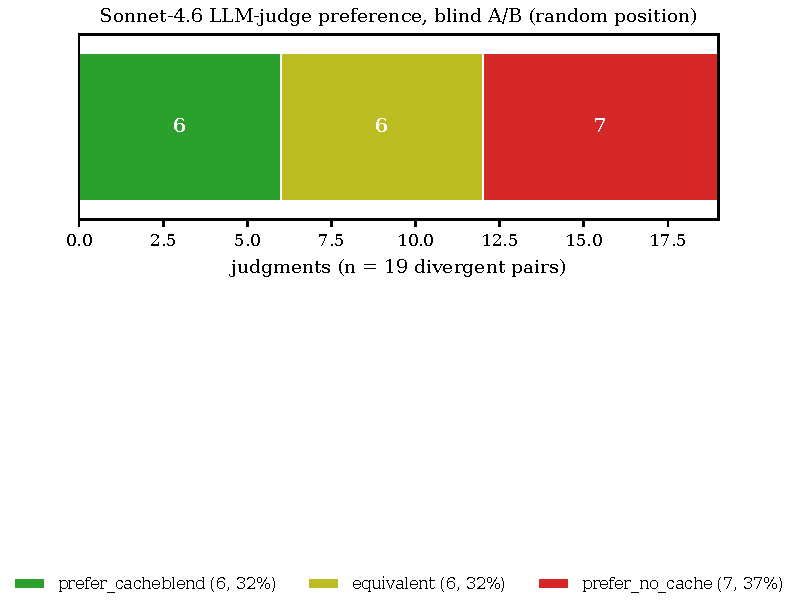
\includegraphics[width=\columnwidth]{figures/judge_summary.pdf}
\caption{Distribution of judge preferences across the 19 divergent
pairs. Equivalent and cacheblend-wins each take 31.6\%; no\_cache-wins
takes 36.8\%. No unparseable judgments.}
\label{fig:judge-summary}
\Description{Horizontal stacked bar chart showing 19 judgments split
into three segments: prefer cacheblend (6, 31.6 percent, green),
equivalent (6, 31.6 percent, olive), and prefer no_cache (7, 36.8
percent, red). No unparseable segment is shown.}
\end{figure}

\paragraph{Per-pair rationales show case-by-case reasoning.}
The per-pair rationales show case-by-case evaluation, not a
mechanical ``prefer tool calls'' heuristic. On
\texttt{swebench\_verified/pytest-7490} turn~3 (no\_cache: tool-call to
a non-existent path; cacheblend: multi-step prose plan), the judge
\emph{prefers cacheblend}: \emph{``Output A provides a more thoughtful,
multi-step plan with multiple relevant tool calls, while Output B
attempts to read a non-existent file path.''} On
\texttt{post\_compact/v6\_align} turn~3, where no\_cache fabricated a
URL-as-filepath while cacheblend ran a working Python demonstration,
the judge again prefers cacheblend. Conversely, on
\texttt{swebench\_verified/astropy-13398} turn~4 (cacheblend: prose
with speculative patch; no\_cache: clean tool call), the judge prefers
no\_cache: \emph{``Output A is a clean, well-formed tool call, while
Output B mixes prose with multiple tool calls and includes a speculative,
likely incorrect patch.''}

The pattern that emerges: cacheblend's blended-KV output is
\emph{sometimes better} than no\_cache's (e.g., when no\_cache picks a
wrong file path and cacheblend's prose plan is more recoverable), but
more often slightly worse, and occasionally catastrophically worse
(the decode-mode flips of \S\ref{sec:eval-identity}). On net, no\_cache
edges cacheblend by 5 percentage points on a 19-pair sample.

\paragraph{Identity rate predicts judge equivalence.} The 28 substantive
bit-identical pairs that we excluded from the judge call (plus the 7
preflight pairs that bypass cacheblend entirely) are trivially
EQUIVALENT; among the 19 judged pairs, the relationship between
token-identity and equivalence persists. All 5 pairs with identity
$\geq$0.5 were judged EQUIVALENT; among the 14 pairs with identity
$<$0.5, the judge returned EQUIVALENT only once. Token-identity is a
strong, near-deterministic predictor of judge equivalence over its
upper half --- below 0.5, real preference signal kicks in. This
matters operationally: a deployment that wants to gate cacheblend
rescue on \emph{measurable} quality preservation can use the
token-identity threshold as a cheap proxy for the judge call, which is
two orders of magnitude more expensive.

\paragraph{Methodological caveats.}
(i) Judge calibration. The multi-judge replication in
Table~\ref{tab:multi-judge} reduces but does not eliminate the
single-judge risk --- all three judges share Anthropic's RLHF
training distribution and could share systematic preferences a
human grader would not have. A human spot-check on a random subset
of the 19 pairs is a sensible next step we do not run here.
(ii) Pairs are dependent (serial sampling within capture), not
independent. The 19 divergent pairs come from 7 captures; pairs from
the same capture share session-cache state, so Wilson CI assumptions
of independence are slightly violated. The CI is reported as-is for
transparency; a clustered bootstrap would tighten it but not change
the headline.
(iii) Conditional vs end-to-end framing. The headline 63.2\% rate is
\emph{conditional} on cacheblend producing a non-bit-identical output
($n_{\text{div}}{=}19$); the end-to-end rate over the 47 substantive
pairs (which folds in the 28 bit-identical pairs as guaranteed
equivalents) is 85.1\%. We do not fold preflight turns back in: rates
of the form $/54$ would mix in pairs where cacheblend never engaged.
(iv) The judge prompt favors tool calls --- intentional calibration to
the agentic context, since CC's wire protocol acts on tool calls and
treats prose as a non-actionable fallback. The judge correctly
preferred prose when the alternative tool call had a wrong
path (pytest-7490 turn~3), suggesting the lean is not pathological.

\subsection{Tool-call vs prose mode agreement}
\label{sec:eval-mode}

A complementary end-to-end view of the agent-protocol cost is whether
the two conditions agree on the model's decode \emph{mode} ---
tool-call (JSON the CC harness can act on) versus prose (which stalls
the agent). For each substantive (capture, turn) pair we classify each
condition's output by whether its first non-whitespace block is a
well-formed function-call JSON. The classifier is a single regex
matching outputs whose leading non-whitespace bytes form a JSON
object containing the keys \texttt{"type": "function"} and
\texttt{"name"}; full regex source is in
\texttt{scripts/dev/extract\_\allowbreak{}tool\_\allowbreak{}call\_\allowbreak{}rate.py}.
This is the same first-block heuristic CC's harness uses to decide
whether to execute a tool call or surface text to the user.

\begin{table}[h]
\small
\centering
\begin{tabular}{lr}
\toprule
Metric over the 47 substantive turns & Rate \\
\midrule
no\_cache tool-call rate              & 30/47 (63.8\%) \\
no\_cache prose rate                  & 17/47 (36.2\%) \\
cacheblend tool-call rate             & 26/47 (55.3\%) \\
cacheblend prose rate                 & 21/47 (44.7\%) \\
\midrule
\textbf{Mode agreement} (NC class $=$ CB class) & \textbf{43/47 (91.5\%)} \\
NC tool-call $\to$ CB prose (\emph{agent stall}) & 4/47 (8.5\%) \\
NC prose $\to$ CB tool-call (recovery) & 0/47 (0.0\%) \\
\bottomrule
\end{tabular}
\caption{Tool-call vs prose mode agreement between no\_cache and
cacheblend, over the 47 substantive pairs of \S\ref{sec:eval-hitrate}'s
corpus. Mode disagreement is \emph{asymmetric}: every disagreement is
cacheblend flipping a tool-call into prose, with no recoveries in the
other direction. The 8.5\% asymmetric stall rate is independent of any
judge-prompt calibration and constitutes a hard floor on cacheblend's
agent-protocol cost on this workload.}
\label{tab:tool-call-mode}
\end{table}

This is the same Mode~A failure mode of \S\ref{sec:eval-identity},
counted directly: blended-KV cacheblend output flips out of tool-call
mode on 4 of the 47 substantive turns where no\_cache would have
produced an actionable tool call. The asymmetry --- zero recoveries
in the prose~$\to$~tool-call direction --- means cacheblend's decode
shift is one-directional and load-bearing for downstream agent
behavior. The 91.5\% mode-agreement rate is consistent with the 85\%
end-to-end non-inferiority rate of \S\ref{sec:eval-judge} (the
difference being that mode agreement counts only protocol form, while
the judge also evaluates argument quality conditional on a matching
mode).

\subsection{Cross-corpus replication on \texttt{skill\_invocation/}}
\label{sec:eval-cross-corpus}

The SWE-V+\texttt{post\_compact} subset (5 SWE-V captures + 2 \texttt{post\_compact/} captures =
$n{=}47$ substantive turns) leaves open whether the findings above
are specific to large-prompt SWE-V-shaped traffic. We replicate the
hit-rate and identity measurements on \dataset's other substantive
subset, \texttt{skill\_invocation/} (1 capture, 53 turns, 52
substantive, max prompt $\sim$2.3k tokens) --- a different workload
shape with shorter prompts and a more uniform skill-preamble
structure. Same backend, same patches, same methodology.

\begin{table*}[t]
\small
\centering
\begin{tabular}{lrrr}
\toprule
Metric & SWE-V+\texttt{post\_compact} subset & \texttt{skill\_inv.} & combined \\
\midrule
$n$ (substantive)              & 47       & 52       & 99 \\
\midrule
\multicolumn{4}{l}{\emph{Rescue rate (\S\ref{sec:eval-hitrate})}} \\
~~median                       & 87.5\%   & 75.4\%   & 76.5\% \\
~~p25                          & 16.1\%   & \textbf{67.9\%} & 67.5\% \\
~~p75                          & 96.8\%   & 95.0\%   & 95.2\% \\
~~$\geq$99\% (steady-state peak) & 6/47 (13\%) & \textbf{0/52 (0\%)} & 6/99 (6\%) \\
~~$\sim$0\% (cold/shift)       & 9/47 (19\%) & 6/52 (12\%) & 15/99 (15\%) \\
\midrule
\multicolumn{4}{l}{\emph{Output identity to no\_cache (\S\ref{sec:eval-identity})}} \\
~~median                       & 1.0000   & 0.8344   & 1.0000 \\
~~bit-identical                & 28/47 (60\%) & 24/52 (46\%) & 52/99 (53\%) \\
~~severe ($<$0.3) divergence   & 14/47 (30\%) & 12/52 (23\%) & 26/99 (26\%) \\
\bottomrule
\end{tabular}
\caption{Same measurements on two \dataset{} subsets and their
union. The qualitative findings replicate; the quantitative shape
of the rescue distribution differs by prompt size in an interpretable
direction.}
\label{tab:cross-corpus}
\end{table*}

\paragraph{What replicates.} The bimodal-with-tail rescue picture,
the order-of-30\% severe-divergence rate, and the
near-50\% bit-identical rate all hold within $\sim$10 percentage
points across the two subsets. The combined-corpus headline numbers
move toward the larger ($n{=}52$) subset's values: median rescue
76.5\%, severe-divergence 26\%, bit-identical 53\%.

\paragraph{What differs by workload shape.} The \texttt{skill\_invocation/}
subset has shorter prompts (max 2.3k tokens vs the SWE-V+\texttt{post\_compact} subset's
4.5--9.5k) and a more uniform within-capture structure (5 skills
$\times$ 3 prompts per skill, cycling). On this workload cacheblend's
rescue distribution \emph{tightens}: the IQR shrinks dramatically
(p25 16.1\%~$\to$~67.9\%) and the steady-state peak vanishes (0/52
turns reach $\geq$99\% rescue, vs 6/47 on §1). The cold-cache tail
also shrinks (19\%~$\to$~12\%). Two structural reasons: (i) shorter
prompts give cacheblend less surface area to either hit perfectly or
miss entirely, so most turns land in the middle band; (ii) the
skill-preamble cycling pattern means each turn's cache LOOKUP tests
against a freshly mixed cache state, never the ``same prompt as
last turn'' steady state where rescue saturates near 100\%.

\paragraph{Implication.} The published 95--99\% cacheblend rescue
peak is not just rare across the SWE-V+\texttt{post\_compact} subset (only 13\% of turns) --- it
appears to be a function of \emph{long, near-duplicate prompts in
sequence}. On workloads dominated by short or structurally-varying
turns it does not appear at all. This sharpens the
``hit rate is not the metric'' thesis: even when rescue \emph{does}
match the published number, it does so on a minority of turns; on
a sibling workload it disappears entirely.

\subsection{Summary}
\label{sec:eval-summary}

The three measurements compose into a single quantitative picture of
cacheblend's tradeoff on Llama-70B fp8 with the \S\ref{sec:patches}
patches:

\begin{itemize}
\item \textbf{Rescue ($n{=}47$ substantive turns):} bimodal --- median
  87.5\%, p25 16.1\%, p75 96.8\%; 13\% of turns reach $\geq$99\%
  steady-state and 19\% sit at $\sim$0\% cold-cache
  (Table~\ref{tab:hit-rate}, Figure~\ref{fig:rescue-distribution}).
\item \textbf{Latency ($n{=}47$):} cacheblend's median TTFT is
  \textbf{55\% slower} than no\_cache (1882\,ms vs 1211\,ms), and
  \textbf{7$\times$ slower} at the $\geq$99\% rescue peak
  (Table~\ref{tab:ttft}, Table~\ref{tab:ttft-by-rescue}). Hit-token
  rescue does not translate to TTFT reduction on this setup.
\item \textbf{Identity ($n{=}47$):} 57\% of substantive turns bit-identical
  to full compute; 30\% diverge severely ($<$0.3 token-identity),
  including 11\% that flip decode mode entirely
  (Figure~\ref{fig:identity-distribution}).
\item \textbf{Agent-protocol usefulness ($n_{\text{div}}{=}19$ divergent
  pairs):} a strong LLM judge prefers cacheblend's output on 31.6\%
  (Wilson CI [15.4\%, 54.0\%]); conditional non-inferiority on the
  divergent pairs is 63.2\%, end-to-end non-inferiority (including the
  28 bit-identical substantive pairs as guaranteed equivalents) is
  85.1\%~/~47 (Table~\ref{tab:judge}, Figure~\ref{fig:judge-summary}).
\item \textbf{Tool-call mode agreement ($n{=}47$):} mode agreement is
  91.5\% but cacheblend asymmetrically flips no\_cache tool-calls into
  prose on 8.5\% of substantive turns (4/47); zero recoveries in the
  other direction (Table~\ref{tab:tool-call-mode}).
\item \textbf{Cross-corpus replication ($n{=}99$, §1 + \texttt{skill\_invocation/}):}
  the bimodal rescue and $\sim$30\% severe-divergence pattern replicates
  on a structurally different second subset, with the $\geq$99\% rescue
  peak vanishing on shorter prompts (0/52 turns on
  \texttt{skill\_invocation/}) and the IQR tightening (p25 jumps
  16\%~$\to$~68\%; Table~\ref{tab:cross-corpus}).
\end{itemize}

Cacheblend's published rescue numbers are reproducible at the
steady-state peak of this distribution but \emph{are not the typical
rescue rate} of natural CC traffic --- the combined-corpus
($n{=}99$) median is 76.5\% with a 15\% cold-cache tail, and the
$\geq$99\% peak appears on only 6\% of turns and is workload-shape
dependent. On the substantive divergent slice where cacheblend's
selective recompute engages non-trivially, the rescued output is
judged non-inferior to a fresh-compute baseline on 63\% of turns,
well below the 85\% spec gate.
\S\ref{sec:discussion} discusses when this trade is acceptable.

% =============================================================================
% Discussion
% =============================================================================

\section{Discussion}
\label{sec:discussion}

\subsection{What this means for deployment}

The headline takeaway from \S\ref{sec:evaluation} is that cacheblend's
rescue is real but not free. On Llama-3.3-70B-Instruct fp8 with our
patches, the rescue is bimodal (median 76.5\% across the main
$n{=}99$ corpus, with 6\% of turns reaching the published 95--99\%
peak; Table~\ref{tab:hit-rate}, Table~\ref{tab:cross-corpus}) ---
and at $T{=}0$, severe ($<$0.3 token-identity to no-cache) divergence
appears on 30\% of substantive turns in the deep-evaluation subset
($n_{\text{sub}}{=}47$) and on 26\% in the combined main corpus
($n{=}99$). On the divergent slice of the deep subset
($n_{\text{div}}{=}19$), an LLM judge prefers cacheblend's output
on only 31.6\% of pairs (Table~\ref{tab:judge}). The asymmetry has
three deployment-relevant implications.

\paragraph{For hit-rate-only workloads, the quality cost is irrelevant
--- but the latency cost still applies.} Any deployment that uses
prefix caching for throughput accounting without surfacing model
outputs directly to end users --- bulk embedding pipelines,
throughput-benchmarking harnesses, KV-cache research itself --- need
not worry about the 30\% divergence: those outputs aren't read. But
the TTFT result of \S\ref{sec:eval-latency} (cacheblend 55\% slower at
median, 7$\times$ slower at peak rescue) still applies: cache hits
are not free latency on a 70B fp8 + H100 backend because LOAD
bandwidth approximately cancels prefill savings. Whether cacheblend
is a net win for these workloads depends on the deployment's
LOAD-to-prefill cost ratio (smaller models, faster interconnect,
slower compute, or throughput-vs-latency optimization all shift the
answer).

\paragraph{For interactive coding agents like Claude Code, the
divergence is load-bearing.} The 37\% no-cache-preferred rate is not a
rounding error: an agent that picks a measurably worse next step on
roughly one in three post-cache turns will surface to end users as
``the cached path is dumber.'' Worse, the failure mode is sometimes a
\emph{decode-mode flip} (tool call$\to$prose, 11\% of substantive
turns); a CC harness that expects a tool-call JSON and receives prose
must either retry, surface a degraded user experience, or silently
fall through. None of these are good outcomes.

\paragraph{For batch RAG-style workloads, the published cacheblend
evaluation remains valid.} Our finding is specific to agent traffic
with multi-turn cache state accumulation; RAG-style workloads where
cache LOOKUP fires once against a single retrieved document set do not
exhibit the same dual-mode divergence pattern. The cacheblend paper's
RAG measurements~\cite{lmcache-cacheblend} are not contradicted by ours.

\subsection{Why agent traffic is harder than RAG for cacheblend}
\label{sec:disc-why-agents}

The cacheblend paper~\cite{lmcache-cacheblend} reports near-100\%
output-quality preservation on permuted-RAG benchmarks at the same
0.15 recompute ratio we use. Our 60\% bit-identity + 30\%
severe-divergence + 8.5\% asymmetric mode-flip rate is a much worse
quality picture on the same mechanism. The 0.15 ratio did not
change; the workload did. We hypothesize three structural reasons,
which we are not yet able to fully ablate but state as testable
hypotheses for follow-up work:

\paragraph{(i) Decode mode is binary in agent traffic, continuous in
RAG.} A RAG response is a prose answer where a small logit
perturbation at position $k$ produces a slightly different word at
position~$k$; the rest of the answer remains semantically close. An
agent response in CC's protocol must commit, within the first $\sim$5
output tokens, to one of two modes: emit \texttt{\{"type":~"function"}
(tool-call) or emit natural-language prose (which the harness cannot
act on). Cacheblend's selective recompute introduces a bounded
logit perturbation, but at position~0 of the output that perturbation
can flip the argmax from \texttt{\{} to \texttt{T}/\texttt{B}/\texttt{L}
(common prose openers). Once a mode is chosen, attention to the
already-emitted prefix reinforces it. RAG outputs do not have this
binary regime sensitivity; agent outputs do, and
\S\ref{sec:eval-mode}'s 8.5\% asymmetric stall rate is the direct
consequence.

\paragraph{(ii) Multi-turn cache accumulation amplifies drift on shared
chunks.} RAG is typically single-turn: retrieve, blend, answer. Agent
traffic is multi-turn, and shared chunks between turns are common ---
the system prompt, repeated tool definitions, and prior conversation
history all appear in successive prompts. \emph{In our replay setup,
prompts are fixed captured request bodies; the model's generated
outputs do not feed back into subsequent prompts.} The drift
accumulation is purely \emph{cache-side}: turn $N$'s STORE writes KV
for the prompt chunks it just processed --- including any chunks
whose KV was itself produced by cacheblend's selective recompute on
turn~$N{-}1$. When turn~$N{+}1$ LOOKUPs a chunk that overlaps with
turn~$N$'s prompt, it retrieves whatever KV turn~$N$ wrote, which
may already be one blending step away from fresh compute. The
cacheblend paper's ``small but bounded'' drift bound applies to each
individual blend operation; we hypothesize that on chunks shared
across multiple consecutive turns the cumulative drift compounds.
This is a hypothesis we have not directly isolated --- a clean test
would require comparing single-turn vs multi-turn replays at fixed
$N$th-turn cache states, which we do not run here.

\paragraph{(iii) Templated prompts have positional dependencies that
permuted-RAG does not.} The cacheblend mechanism is most accurate when
the model's attention to a chunk is approximately invariant to that
chunk's exact position --- permuted-RAG, by construction, trains on
this kind of invariance. CC's prompts are highly templated (system
prompt with tool list at fixed offsets, conversation history in
chronological order, current user message at a known position) and the
model has learned strong position-conditioned patterns. When
cacheblend re-uses a cached chunk at a new position, the chunk's KV
reflects attention computed in the \emph{original} positional context,
and the selective-recompute correction sees only 15\% of layers
through the new positional context. For position-sensitive templates
the residual drift on the un-recomputed 85\% of layers compounds; for
permuted-RAG it largely cancels.

Hypothesis~(iii) is directly testable: at
\texttt{LMCACHE\_BLEND\_\allowbreak{}RECOMPUTE\_RATIOS}=1.0, every layer
is recomputed in the new positional context, so the un-recomputed
residual vanishes and identity to no\_cache should recover. We test
this directly in \S\ref{sec:disc-knobs} and find it does. Hypotheses
(i)~and (ii) remain open empirical questions for future work.

\subsection{Recompute-ratio sweep tests hypothesis (iii)}
\label{sec:disc-knobs}

To probe hypothesis~(iii) of \S\ref{sec:disc-why-agents} ---
residual drift on the un-recomputed layers --- we sweep
\texttt{LMCACHE\_BLEND\_\allowbreak{}RECOMPUTE\_RATIOS} over
$\{0.15, 0.5, 1.0\}$ on the
\texttt{swebench\_verified/\allowbreak{}pytest-7490} fixture (4
turns, 3 substantive at $\geq$256 prompt tokens, samples=1, otherwise
identical to the SWE-V+\texttt{post\_compact} subset methodology):

\begin{table}[h]
\small
\centering
\begin{tabular}{lrrr}
\toprule
Ratio & Mean token-identity to NC & Aggregate rescue \% \\
\midrule
\textbf{0.15 (default)} & 0.847 & 27.4\% \\
0.50                    & 0.831 & 27.4\% \\
\textbf{1.00}           & \textbf{1.000} & 27.4\% \\
\bottomrule
\end{tabular}
\caption{Recompute-ratio sweep on \texttt{pytest-7490} ($n{=}3$
substantive turns per ratio). Identity to the no\_cache baseline
recovers to 1.000 at ratio=1.0 (every layer recomputed in the new
positional context) but stays around 0.83 at the intermediate ratio,
not 0.92 as one would extrapolate. Rescue percent is unchanged because
\texttt{RECOMPUTE\_RATIOS} controls layer recompute, not which KV
tokens are loaded from cache.}
\label{tab:recompute-sweep}
\end{table}

Two findings:

\paragraph{Hypothesis (iii) is supported.} At ratio=1.0, identity to
\texttt{no\_cache} recovers bit-perfectly. Recomputing every layer in
the new positional context eliminates the residual drift that the
default 0.15 ratio carries. The mechanism we hypothesized in
\S\ref{sec:disc-why-agents}(iii) is the load-bearing one for the
identity gap.

\paragraph{Partial recompute did not partially recover on this
probe.} Going from $0.15 \to 0.5$ (3.3$\times$ more layers recomputed)
barely moves identity (0.847~$\to$~0.831), within noise on $n{=}3$.
Recovery is concentrated at the discrete $\to{}1.0$ jump on the data
points we have. \emph{We do not claim the intermediate-ratio tradeoff
curve is established from $n{=}3$:} a larger sweep (denser ratio grid
$\times$ the full deep-evaluation subset) is needed before
concluding that no monotonic recovery exists between 0.15 and 1.0.
What is robust from this probe is the discrete endpoint contrast:
ratio~1.0 produces identity~$=$~1.000 by construction (every layer
recomputed in the new positional context), confirming the
positional-context hypothesis. Whether 0.5 or 0.8 would offer a
useful Pareto-improvement remains an open question.

The combination of \S\ref{sec:eval-latency}'s TTFT measurement
(cacheblend already slower than \texttt{no\_cache} at the default
0.15 ratio on our backend) and this sweep's discrete-jump pattern
suggests cacheblend's default ratio is not clearly a good operating
point in our measurements, and that ratio=1.0 may not be the
practical fix (it recomputes every layer, eliminating the rescue
benefit). A genuine graded tradeoff curve --- one that gives
proportional identity recovery against linear cost --- may require
mechanism changes beyond the existing recompute-ratio knob
(smaller cacheable blocks, layer-importance-aware recompute
selection, or model-architecture co-design are candidates worth
exploring).

\paragraph{Sample size caveat.} Three substantive turns per ratio is
a small sample; the 0.847~$\to$~0.831 dip at 0.5 is plausibly noise.
What is robust is the discrete jump at 1.0 from $\sim$0.84 to exactly
1.000 --- that comes from the math, not the sample. A larger probe
across the full SWE-V+\texttt{post\_compact} subset would tighten the intermediate-ratio
identity estimates but is unlikely to change the discrete
0.15$\leftrightarrow$1.0 endpoint contrast.

\subsection{Resource-constrained methodology choices}
\label{sec:disc-resource}

This paper was produced on a fixed compute budget (\$25 envelope for
the headline experiments, against a 2$\times$ H100 80GB SXM pool with
real per-pod cost). Several methodological tightenings a reviewer
would reasonably ask for --- a raw-no-cache baseline that bypasses our
parser to validate separator injection is content-neutral, an
intra-condition repeatability study to bound run-to-run
nondeterminism, instrumented per-phase TTFT breakdowns (LMCache
LOAD vs prefill vs blend vs scheduler vs decode), a denser
recompute-ratio grid, a quantitative patch ablation that runs each
intermediate configuration as its own pod replay, and a bf16-vs-fp8
precision comparison --- are individually small but cumulatively a substantial increase in
pod-hours, well beyond this project's compute budget. We list them
explicitly as open empirical questions rather than implicit ones, so
that a reader who wants to commission this work knows where it sits
relative to our existing claims. The headline findings (rescue is
bimodal, identity gap is real, latency cost is real, mode-flip
asymmetry is real) are robust to the methodology gaps we name here ---
they are direct read-offs from the measurements we did run, not
inferences that depend on the missing instrumentation. The
\emph{causal} explanations for those findings are where the missing
instrumentation would matter most; we have flagged each one as a
hypothesis rather than a conclusion.

\subsection{Limitations}
\label{sec:disc-limits}

\textbf{Single model.} All measurements are on Llama-3.3-70B-Instruct
fp8. The cacheblend mechanism is model-agnostic in design, but the
empirical quality cost is not: the fp8 quantization noise floor, the
70B parameter count, and Llama's attention architecture all interact
with cacheblend's selective recompute. The same patches and methodology
on Sonnet, Haiku, Llama-8B, or Qwen could produce a different
divergence distribution. \S\ref{sec:disc-knobs}'s recompute-ratio probe
is the higher-priority follow-up; multi-backend characterization
is the longer-horizon next step.

\textbf{Judge calibration.} We replicate the 19-pair A/B against
Opus-4.7 and Haiku-4.5 in \S\ref{sec:eval-judge}, and the
three-judge majority vote reproduces Sonnet-4.6's headline numbers
(31.6\% preference, 63.2\% non-inferior). The single-judge risk is
reduced but not eliminated --- all three judges share Anthropic's
RLHF training, so a coordinated calibration bias could still apply.
A human spot-check is a sensible next step we do not run here.

\textbf{Single decoding temperature.} $T=0$ greedy decoding makes
single-token differences load-bearing: a divergence at position $k$
permanently forks the trajectory. Sampling at $T=0.7$ would average
over multiple plausible continuations and might mask or amplify the
cross-condition divergence in the marginal distribution. We defer
the $T>0$ distributional measurement to follow-up work.

\textbf{Sample size.} 19 divergent pairs is small. The 95\% Wilson CI
on the cacheblend preference rate spans [15.4\%, 54.0\%] --- we cannot
reject ``cacheblend is preferred half the time'' from the data alone.
The point estimate's location well below 50\% is what supports the
non-inferiority gate failing; widening the corpus would tighten the
interval but is unlikely to change the qualitative direction.

\textbf{Workload diversity within \dataset{}, but a single corpus
source.} The combined $n{=}99$ corpus mixes SWE-bench-Verified
sessions, \texttt{post\_compact/} canonical captures, and
\texttt{skill\_invocation/} (\S\ref{sec:eval-cross-corpus}). All three
subsets come from one researcher's laptop running one client family
(CC SDK), so the captured prompt distribution is not yet broad across
operators, languages, or task domains. The cross-corpus replication
of the bimodal-rescue and severe-divergence patterns supports
generality \emph{within Claude-Code-shaped traffic}; we make no claim
about other agent harnesses (Cursor, Aider, OpenAI Codex, etc.) on
this evidence alone.

\textbf{Backend specificity.} All measurements use a
Llama-3.3-70B-Instruct fp8 backend on 2$\times$ H100 80GB SXM, vLLM
v0.19.0, and lmcache v0.4.2 with our patches. We do not claim
generality across smaller models, different precisions (bf16),
faster interconnects, or non-vLLM serving stacks. The bf16 vs fp8
comparison is the highest-priority open empirical question;
\S\ref{sec:disc-knobs}'s recompute sweep already isolates one
hypothesis on the present backend.

\subsection{Recommendation}
\label{sec:disc-recommend}

We make one concrete methodological recommendation:
\emph{KV-cache reuse research should report output-quality measurements
alongside hit-rate measurements, on at least one agentic workload, with
a structured methodology that includes $T=0$ token-identity and a
strong-judge blind A/B preference test.} The hit-rate-only framing
that the field has converged on is sufficient for the RAG-style
workloads the early prefix-caching literature targeted, but it
silently elides exactly the failure mode we surface here: a mechanism
can hit at the published rate and still produce systematically worse
output on the same input. We provide \dataset{} and the \sys{} harness
as the reproducible substrate for this kind of evaluation.

% =============================================================================
% Related Work
% =============================================================================

\section{Related Work}
\label{sec:related}

\paragraph{LLM serving infrastructure.}
vLLM~\cite{vllm-sosp} introduced paged-attention KV caching as a
production-grade serving substrate; SGLang~\cite{sglang-paper} extended
the paged-attention idea with RadixAttention's tree-structured prefix
sharing; TGI~\cite{tgi-repo} and DistServe~\cite{distserve-osdi}
explored complementary directions in batching and disaggregated
prefill/decode. \sys{} layers on top of vLLM and reuses its
paged-attention prefix cache without modification; our contribution is
at the proxy and cross-request integration layer, not at the inference
kernel.

\paragraph{KV cache reuse and prefix caching.}
The closest prior work is the LMCache + cacheblend
line~\cite{lmcache-paper, lmcache-cacheblend}, which provides the
cross-request KV store and the selective-recompute mechanism that \sys{}
integrates. Prompt Cache~\cite{promptcache-mlsys} addressed a similar
problem from the compiler-IR direction (statically-analyzable prompt
templates), and ChunkAttention~\cite{chunkattention} extended
prefix-sharing to the attention computation itself. None of these prior
systems target Anthropic-shaped agent traffic, and none measure the
output-quality cost of their reuse mechanism on a non-RAG workload.
Our contribution against this thread is twofold: (a) the patches and
proxy needed to actually run cacheblend against natural CC traffic on a
non-toy backend (\S\ref{sec:patches}), and (b) the quality-versus-rescue
characterization in \S\ref{sec:evaluation} that the published cacheblend
evaluation did not surface.

\paragraph{LLM agent benchmarks.}
SWE-bench~\cite{swe-bench-iclr} and its curated variant
SWE-bench Verified~\cite{swe-bench-verified} provide the canonical
task suite for agentic coding evaluation; MetaGPT~\cite{metagpt-paper}
and AgentBench~\cite{agentbench} extend the agent-benchmark surface to
multi-agent and multi-domain settings. These benchmarks all measure
\emph{end-task success}: did the agent close the bug, pass the tests,
write the working code. \dataset{} is complementary, not a replacement
--- it measures \emph{traffic-shaped} serving-system properties (cache
hit rate, output identity, judge preference) on captures of CC sessions
that themselves work on SWE-V tasks. A serving-system paper can use
\dataset{} to benchmark cache strategy; an agent-quality paper still
needs SWE-V (or successor) to measure task success.

\paragraph{Output-quality evaluation.}
MT-Bench~\cite{mtbench}, AlpacaEval~\cite{alpacaeval}, and Chatbot
Arena~\cite{chatbot-arena} established LLM-as-judge as a credible
methodology for ranking model outputs. We apply the same methodology
in a different setting --- not to rank candidate \emph{models} on the
same input, but to rank the outputs of the same model under different
\emph{cache strategies}. The position-randomization and
prompt-caching elements of our setup follow the
MT-Bench~\cite{mtbench} recipe. We additionally run three-judge
replication (Sonnet-4.6 / Opus-4.7 / Haiku-4.5;
Table~\ref{tab:multi-judge}) and find that the majority-vote
verdict reproduces the single-judge headline rates exactly, which
is consistent with the cited works' observation that multi-judge
consensus is a strict improvement over single-judge ranking but the
calibration gap is small when the divergent-pair sample is well
separated.

% =============================================================================
% Conclusion
% =============================================================================

\section{Conclusion}
\label{sec:conclusion}

We presented \sys{}, a transparent proxy (drop-in for Claude Code
clients given a patched lmcache backend) that integrates cacheblend
with Claude-Code-shaped traffic replayed on a Llama-3.3-70B fp8 +
vLLM + LMCache backend; \dataset{}, a benchmark of 13 captures /
182 turns / 411k tokens of redacted on-wire CC request bodies; and,
to our knowledge, the first measurement of cacheblend's
agent-protocol usefulness cost on natural agent traffic at this
backend scale. Across two corpus subsets (combined $n{=}99$
substantive turns) cacheblend rescues a median 76.5\% of prefill
tokens; the published 95--99\% steady-state peak appears on only
6\% of turns and disappears entirely on the
\texttt{skill\_invocation/} workload
(Table~\ref{tab:hit-rate}, Table~\ref{tab:cross-corpus}). The rescue
is not free: at $T{=}0$, 30\% of substantive turns produce severely
divergent output (Sonnet-4.6 judge analysis on the divergent slice
$n_{\text{div}}{=}19$ from the SWE-V+\texttt{post\_compact} subset:
31.6\% prefer cacheblend, 63.2\% conditional non-inferiority versus an
85\% pre-registered gate; Opus-4.7 and Haiku-4.5 majority-vote
replicates Sonnet exactly; Table~\ref{tab:judge},
Table~\ref{tab:multi-judge}).

Our methodological claim is independent of the patches:
\emph{hit rate is not output quality, and a KV-cache reuse
mechanism that hits at the published rate while producing
systematically different output on the same input is not the same
artifact}. \sys{} and \dataset{} are the substrate for asking that
second question on agent-shaped workloads.

\paragraph{Availability.} \dataset{} is available now at
\url{https://huggingface.co/datasets/intelchen/claudecode-trace}
under CC-BY 4.0. The dataset contains redacted CC outbound request
bodies (\S\ref{sec:dataset-redact}) collected from the lead author's
own usage of Claude Code; redaction removes Tailscale/HF/RunPod
credentials, local filesystem paths, and the CC client account
identifier. Anthropic Claude Code is closed-source proprietary
software; the redacted captures themselves are released as factual
recordings of the wire protocol (analogous to network capture
fixtures), which we believe is consistent with CC's terms of
service for non-derivative research use, but we make no legal
warranty.
\sys{} source, the patched lmcache wheel, the bench harness, and
the figure-generation scripts will be released on acceptance under
MIT license. For double-blind review, a frozen submission-time tag
is accessible via an anonymous Zenodo archive linked from the
submission. The
\texttt{scripts/dev/\allowbreak{}extract\_\allowbreak{}full\_\allowbreak{}corpus\_\allowbreak{}rescue.py}
and \texttt{extract\_\allowbreak{}tool\_\allowbreak{}call\_\allowbreak{}rate.py}
drivers used for the quantitative tables in \S\ref{sec:evaluation}
are part of that artifact and re-run end-to-end against the public
\dataset{}.


\bibliographystyle{ACM-Reference-Format}
\bibliography{refs}

% =============================================================================
% Appendix
% =============================================================================

\appendix

\section{Judge Prompt Template}
\label{app:judge-prompt}

The Sonnet-4.6 judge in \S\ref{sec:eval-judge} is invoked with a
fixed system prompt and a per-pair user message whose A/B ordering is
randomized per call. The full templates appear below verbatim;
the implementation lives in
\texttt{src/skillcacher/judge/prompt.py}.

\paragraph{System prompt.}
\begin{quote}\footnotesize\itshape
You are evaluating two outputs from an AI coding agent. The agent is
operating in an interactive multi-turn task where it uses tool calls
(JSON function-call blocks) to read files, edit code, and make
progress on software-engineering tasks.

Both outputs are responses from the SAME agent context to the SAME
prompt --- the only difference is the engine's KV-cache strategy.
Your job is to identify which output is a better next step for the
agent's task.

When comparing:
\begin{itemize}
\item A well-formed tool call (JSON specifying a function name +
  arguments) is generally better than natural-language prose,
  because the agent's task requires tool calls to make progress.
\item When both outputs are tool calls, prefer the one with more
  appropriate arguments --- sensible file paths, reasonable command
  flags, useful descriptions.
\item When both outputs are prose, prefer the one that more directly
  addresses the task.
\item If the outputs are functionally equivalent (e.g., same tool
  with cosmetically different argument wording), respond
  \texttt{EQUIVALENT}.
\end{itemize}

Respond with EXACTLY one of these tokens on the first line:
\texttt{PREFER\_A} \textbar{} \texttt{PREFER\_B} \textbar{} \texttt{EQUIVALENT}.
Then on a new line, give a 1-sentence rationale ($\leq$ 30 words).
\end{quote}

\paragraph{User template.} Rendered per pair with the task prompt
and both outputs substituted:
\begin{lstlisting}[basicstyle=\ttfamily\footnotesize, frame=single,
                   framesep=4pt, breaklines=true]
TASK PROMPT (what the agent was asked to do):
{task_prompt}

OUTPUT A:
{output_a}

OUTPUT B:
{output_b}
\end{lstlisting}

\paragraph{Parsing.} Responses are parsed with the line-anchored
regex \texttt{\^{}\textbackslash{}s*(PREFER\_A|PREFER\_B|EQUIVALENT)\textbackslash{}b}
applied in multiline mode. The label is mapped back to
\{cacheblend, no\_cache, equivalent\} via the recorded
\texttt{position\_a} for that call; anything that does not match the
regex on either of the first two lines is recorded as
\texttt{UNPARSEABLE} (zero occurrences across the 19-pair run).
Rationales are extracted as the remainder of the response after the
label token, trimmed and truncated at the first newline.

\paragraph{Calling conventions.} The judge is invoked via the
Anthropic Messages API with top-level \texttt{cache\_control:
\{type: "ephemeral"\}} on the static system prompt; per-pair user
messages bypass the cache. Position assignment is seeded
per pair (\texttt{random.Random(42 \^{} hash((capture\_id,
turn\_index)))}) so that re-running the judge call deterministically
reproduces both the A/B ordering and any cache hits on the system
prompt.

\section{Statistical Span Miner}
\label{app:miner}

The miner extracts repeated token sequences from the
\dataset{} corpus for the pre-seed dispatcher
(\S\ref{sec:miner}). Inputs: a list of token streams (one per
captured request). Parameters: a length floor
$\ell_{\min}$=256~tokens (matching
\texttt{lmcache.blend\_min\_tokens}), a frequency floor
$f_{\min}$=3~distinct streams, a MinHash Jaccard cutoff $J$=0.8,
and a shingle width $k$=5. The output is a list of
\texttt{MinedSpan} records, sorted by
$(\text{frequency descending}, \text{length descending})$, each
carrying its token ids, originating stream ids, and frequency
count. The reference implementation
(\texttt{src/\allowbreak{}skillcacher/\allowbreak{}tagging/\allowbreak{}statistical\_\allowbreak{}miner.py},
$\sim$340 LoC) follows the procedure below.

\begin{algorithm}[h]
\small
\textbf{Inputs:} streams $S_1, \dots, S_m$;
                 $\ell_{\min}$, $f_{\min}$, $J$, perms $P$, shingle width $k$.\\
\textbf{Output:} sorted list of mined spans.

\begin{enumerate}
  \item[1.] \emph{Concatenate.} Build $T = S_1 \cdot \sigma_1 \cdot S_2 \cdot \sigma_2 \cdots S_m$
    where each $\sigma_i$ is a unique negative sentinel that prevents
    suffixes from crossing stream boundaries. Maintain a parallel
    array \texttt{stream\_of\_pos} mapping each position to its
    originating stream id.

  \item[2.] \emph{Suffix array via prefix doubling.} Compute
    $\mathrm{SA}[0\,..\,n{-}1]$ such that $\mathrm{SA}[i]$ is the
    starting index of the $i$-th lex-smallest suffix of $T$. Each
    round sorts on the composite key
    $(\mathrm{rank}[i], \mathrm{rank}[i{+}k])$, doubling $k$ each
    iteration; terminates when all ranks are unique. Total work
    $O(n \log^2 n)$, memory $O(n)$. (The naive sort by full suffix
    string is $O(n^2)$ in expectation on this corpus and was
    benchmarked to hang on $n {\geq} 250\mathrm{K}$.)

  \item[3.] \emph{Kasai LCP.} Compute $\mathrm{LCP}[i]$ = length of
    the longest common prefix of $\mathrm{SA}[i{-}1]$ and
    $\mathrm{SA}[i]$ in linear time via the Kasai
    algorithm~\cite{kasai-lcp}.

  \item[4.] \emph{Monotonic-stack enumeration of maximal repeats.}
    Sweep $\mathrm{LCP}$ left-to-right with a stack of
    $(\text{height}, \text{left\_index})$ pairs. For every entry that
    pops because the current LCP dips below it, emit
    $\mathrm{SA}[\text{left\_index}{-}1\,..\,i{-}1]$ as a candidate of
    length \text{height}: those suffixes share at least
    $\text{height}$ characters. This enumerates the nested case
    (a 350-token repeat at freq=3 nested inside a 300-token repeat
    at freq=5 emits both).

  \item[5.] \emph{Floor + sentinel filters.} Discard candidates with
    length $< \ell_{\min}$, with fewer than $f_{\min}$ distinct
    source streams (computed via \texttt{stream\_of\_pos}), or
    containing any sentinel token (negative id). Deduplicate by
    fingerprint hash.

  \item[6.] \emph{Exact-prefix dedup.} Sort surviving candidates by
    length descending. If candidate $A$'s tokens are a prefix of an
    already-kept candidate $B$ with $|A| < |B|$ and they share at
    least one source stream, drop $A$ ($B$ is strictly more
    informative).

  \item[7.] \emph{MinHash near-dup dedup.} Compute a $P$-permutation
    MinHash signature over $k$-shingles for each remaining span. Two
    spans whose signature Jaccard $\geq J$ are merged, keeping the
    longer representative. We use $P{=}64$, $k{=}5$, $J{=}0.8$; the
    blake2b-keyed hash family makes the signatures deterministic
    across runs and tractable on 64-bit machines.

  \item[8.] \emph{Sort + return.} Sort by
    $(-\text{frequency}, -\text{length})$ so callers can take the
    top-$N$ under a budget cap.
\end{enumerate}
\caption{\texttt{mine\_spans}: extract length-$\geq{}\ell_{\min}$,
frequency-$\geq{}f_{\min}$ near-deduped repeated sequences from
a multi-stream token corpus.}
\label{alg:miner}
\end{algorithm}

\paragraph{Empirical scale.} On the union of
\dataset's three subsets (411k tokens, 182 streams) with
$\ell_{\min}=256$, $f_{\min}=3$, $J=0.8$, the miner returns
\textbf{181 spans totalling 278k tokens}, in approximately 18~s on
a single MacBook Pro core. The top hit is a 1{,}691-token span
occurring in 26 of the 182 streams (the CC system prompt with tool
list); the long tail of mid-frequency spans corresponds to repeated
skill preambles and tool-output formatting blocks.

\section{Reproducibility}
\label{app:reproducibility}

\paragraph{Pod configuration.} All \S\ref{sec:evaluation} measurements
use a single pod recipe: \mbox{2$\times$~NVIDIA~H100~80GB} on RunPod's
\texttt{SECURE} cloud, vLLM v0.19.0 with the
\texttt{LMCacheConnectorV1} attached, lmcache v0.4.2 with the
patches in \S\ref{sec:patches}, model
\texttt{meta-llama/Llama-3.3-70B-\allowbreak{}Instruct} loaded at
\texttt{dtype=fp8}, tensor-parallel degree~2, and
\texttt{max\_model\_len=32768}. The cacheblend condition additionally
exports the eight \texttt{LMCACHE\_*} environment variables in
Table~\ref{tab:repro-env}; \texttt{PYTHONHASHSEED=0} is mandatory
for chunk-hash stability across the connector's per-role
\texttt{TokenDatabase} inits.

\begin{table}[t]
\small
\centering
\begin{tabular}{ll}
\toprule
Variable & Value \\
\midrule
\texttt{PYTHONHASHSEED} & \texttt{0} (required) \\
\texttt{VLLM\_KV\_CACHE\_TYPE} & \texttt{lmcache} \\
\texttt{LMCACHE\_USE\_EXPERIMENTAL} & \texttt{True} \\
\texttt{LMCACHE\_LOCAL\_CPU} & \texttt{True} \\
\texttt{LMCACHE\_MAX\_LOCAL\_CPU\_SIZE} & \texttt{40} \\
\texttt{LMCACHE\_CHUNK\_SIZE} & \texttt{256} \\
\texttt{LMCACHE\_ENABLE\_BLENDING} & \texttt{True} \\
\texttt{LMCACHE\_USE\_LAYERWISE} & \texttt{True} \\
\texttt{LMCACHE\_BLEND\_SPECIAL\_STR} & \texttt{" \# \# "} \\
\texttt{LMCACHE\_BLEND\_CHECK\_LAYERS} & \texttt{1} \\
\texttt{LMCACHE\_BLEND\_RECOMPUTE\_RATIOS} & \texttt{0.15} (default) \\
\bottomrule
\end{tabular}
\caption{Environment variables for the \texttt{cacheblend} condition.
Set on the pod before \texttt{vllm serve} is launched. Omitting any
of the eight \texttt{LMCACHE\_*} variables causes the engine either
to crash at startup or to silently fall through to plain prefix
caching (no rescue).}
\label{tab:repro-env}
\end{table}

\paragraph{Provisioning resilience.} RunPod's 2$\times$~H100 pool is
capacity-tight enough that synchronous HTTP 500 ``no instances
available'' rejections at \texttt{POST /pods} are routine. We
combine three mitigations: (i) \texttt{CLOUD\_TYPE=SECURE} with
\texttt{WAIT\_TIMEOUT\_S=3600} and
\texttt{PROVISIONING\_TIMEOUT\_S=1800} to let an accepted pod queue
patiently for hardware; (ii) a bash retry loop around the
\texttt{skillcacher-bench} invocation for synchronous create
rejections (20 attempts, 120~s sleep between); (iii) sequential
execution of multi-condition runs so the harness cannot multiply
its own capacity demand. The
\texttt{scripts/dev/recompute\_probe.sh} driver in our repository is
the canonical example.

\paragraph{Canonical commands.} The complete SWE-V+\texttt{post\_compact} subset replay
(7~captures, 54~pairs across three conditions) is one invocation:
\begin{lstlisting}[basicstyle=\ttfamily\scriptsize, frame=single,
                   framesep=4pt, breaklines=true]
SKILLCACHER_BACKEND_MAX_COMPLETION_TOKENS=512 \
MODEL_NAME=meta-llama/Llama-3.3-70B-Instruct \
DTYPE=fp8 GPU_COUNT=2 TENSOR_PARALLEL_SIZE=2 \
MAX_MODEL_LEN=32768 CLOUD_TYPE=SECURE \
WAIT_TIMEOUT_S=3600 PROVISIONING_TIMEOUT_S=1800 \
skillcacher-bench quality-eval \
  --corpus-dir tests/fixtures/claude_code_real \
  --capture-filter \
"swebench_verified/{astropy-13398,matplotlib-26113,\
pylint-7080,pytest-7490,sphinx-11510},\
post_compact/plan4_compaction_spike_v{6_align,7_norm}" \
  --conditions no_cache,prefix_cache,cacheblend \
  --samples 1 --temperature 0 \
  --out benchmark/results/plan5_quality_section1
\end{lstlisting}
The judge analysis is then a single offline invocation reading
the parquets emitted by the above:
\begin{lstlisting}[basicstyle=\ttfamily\scriptsize, frame=single,
                   framesep=4pt, breaklines=true]
export $(grep -E "^ANTHROPIC_API_KEY=" .env | xargs)
.venv/bin/python scripts/run_judge.py --skip-identical
\end{lstlisting}

\paragraph{Artifact availability.} Three artifacts support
end-to-end reproduction. (i)~\dataset{} on Hugging
Face~\cite{claudecode-trace-hf}, available now under CC-BY 4.0; the
\texttt{scripts/download\_claudecode\_trace.py} wrapper accepts
\texttt{--subset} filters. (ii)~\sys{} source, including the
patched lmcache wheel build script, the proxy, the bench harness,
and the figure-generation scripts; the analysis drivers used for
\S\ref{sec:eval-hitrate} and \S\ref{sec:eval-mode}
(\texttt{scripts/dev/extract\_\allowbreak{}full\_\allowbreak{}corpus\_\allowbreak{}rescue.py},
\texttt{scripts/dev/extract\_\allowbreak{}tool\_\allowbreak{}call\_\allowbreak{}rate.py})
are part of this set. (iii)~The pod-orchestration driver
(\texttt{scripts/dev/oneshot\_pod.\{sh,py\}}) and the recompute-ratio
sweep driver (\texttt{scripts/dev/recompute\_probe.sh}). Items
(ii)~and~(iii) are released under MIT on acceptance, with a frozen
submission-time tag accessible to reviewers via a double-blind-
compatible anonymous Zenodo archive linked from the submission.

\section{Anchor Recognition Walkthrough}
\label{app:anchors}

To make \S\ref{sec:cc-segment}'s parser concrete, this appendix shows
one real CC request body (lightly redacted) with the structural
anchors color-highlighted and the cacheblend separator
\texttt{\textquotedbl{}~\#~\#~\textquotedbl{}} marked at each
injection site.

\definecolor{anchorHeader}{HTML}{FFF3B0}   % header (normalized fields)
\definecolor{anchorGit}{HTML}{B8E0F5}      % gitStatus
\definecolor{anchorCommits}{HTML}{F8C8DC}  % recent commits
\definecolor{anchorReminder}{HTML}{D4EFCE} % system-reminder

\paragraph{Color key.}
\colorbox{anchorHeader}{\strut\,header\,} (per-turn, normalized
per \S\ref{sec:header-norm});
\colorbox{anchorGit}{\strut\,gitStatus\,};
\colorbox{anchorCommits}{\strut\,commits\,};
\colorbox{anchorReminder}{\strut\,\texttt{<system-reminder>}\,}.
The injected separator is shown as
\fbox{\,\texttt{~\#~\#~}\,} between blocks; cacheblend treats
each separated span as one chunk for STORE / LOOKUP / blend.

\begin{figure}[h]
\begin{flushleft}\small\ttfamily
\fbox{\,\texttt{~\#~\#~}\,}\\[1pt]
\colorbox{anchorHeader}{\strut\,x-anthropic-billing-header:
cc\_version=NORM; cch=NORM;\,}\\
\fbox{\,\texttt{~\#~\#~}\,}\\[1pt]
CWD: /Users/$\langle$user$\rangle$/skillcacher\\
Date: 2026-05-08\\[3pt]
\colorbox{anchorGit}{\strut\,gitStatus: This is the git status\dots\,}\\
\colorbox{anchorGit}{\strut\,Current branch: main\,}\\
\colorbox{anchorGit}{\strut\,Status:\,}\\
\colorbox{anchorGit}{\strut\,M~~benchmark/results/audit/$\dots$\,}\\
\colorbox{anchorGit}{\strut\,??~scripts/dev/cacheblend\_quality.sh\,}\\
\fbox{\,\texttt{~\#~\#~}\,}\\[1pt]
\colorbox{anchorCommits}{\strut\,Recent commits:\,}\\
\colorbox{anchorCommits}{\strut\,f8a0cfa fix(capture): plant\dots\,}\\
\colorbox{anchorCommits}{\strut\,12778ec docs: Plan 3 resume\dots\,}\\
\fbox{\,\texttt{~\#~\#~}\,}\\[1pt]
\colorbox{anchorReminder}{\strut\,$\langle$system-reminder$\rangle$\,}\\
\colorbox{anchorReminder}{\strut\,As you answer the user's
questions\dots\,}\\
\colorbox{anchorReminder}{\strut\,$\langle$/system-reminder$\rangle$\,}\\
\fbox{\,\texttt{~\#~\#~}\,}\\[1pt]
\end{flushleft}
\caption{One real CC request, anchors highlighted. The parser
identifies four blocks: the per-turn billing header (yellow), the
gitStatus block (blue), the Recent-commits block (pink), and the
\texttt{<system-reminder>} wrapper (green). Cacheblend separators
are injected on each side of every recognized block. The yellow
block's \texttt{cc\_version} and \texttt{cch} fields have already
been rewritten to \texttt{NORM} by \S\ref{sec:header-norm}'s
header normalizer, which is why the first KV chunk's hash is
stable across multi-turn sessions.}
\label{fig:anchor-walkthrough}
\Description{Color-highlighted representation of a Claude Code
request body. Four anchor classes are marked: yellow for the
per-turn billing header, blue for the gitStatus block, pink for
Recent commits, and green for the system-reminder wrapper.
Cacheblend separator markers shown as boxed double-pound symbols
between each anchor block.}
\end{figure}

\paragraph{What the parser does at each anchor.}
\begin{enumerate}
\item \textbf{Per-turn header (yellow):} detected by the
  \texttt{x-anthropic-\allowbreak{}billing-\allowbreak{}header:}
  prefix. The \texttt{cc\_version} and \texttt{cch} field values
  are rewritten
  in place to \texttt{NORM} placeholders before chunk hashing, so
  the first KV chunk hash is identical across all turns of one CC
  session (\S\ref{sec:header-norm}).
\item \textbf{gitStatus (blue):} detected by the literal
  \texttt{gitStatus:\textbackslash{}n} prefix. Typically 100--400
  tokens long; spans the working-tree summary CC injects on session
  start. Content is stable for the lifetime of a session.
\item \textbf{Recent commits (pink):} detected by
  \texttt{Recent commits:\textbackslash{}n}. Typically 50--200
  tokens; the most recent commit hashes drift across sessions but
  the structural anchor is stable.
\item \textbf{\texttt{<system-reminder>} wrapper (green):} detected
  by the literal tag pair. Variable-length (30--200 tokens
  typically), often falls below
  \texttt{blend\_min\_tokens}=256 in isolation and is rolled into
  an adjacent block rather than getting its own separator pair ---
  see \S\ref{sec:cc-segment}.
\end{enumerate}

\paragraph{Why this matters.} Without the parser, cacheblend's
default \texttt{blend\_special\_str=\textquotedbl{}~\#~\#~\textquotedbl{}}
never appears in CC outbound traffic --- CC's wire format uses
\texttt{\textbackslash{}n\textbackslash{}n} as its block delimiter,
and the resulting 25--180-token spans fall under the 256-token
floor. The parser's job is to inject the configured separator at
exactly the boundaries that produce content-stable, $\geq$256-token
chunks. The four highlighted classes above are what enables
cacheblend to engage at all on natural CC traffic.


\end{document}
